\documentclass[conference, compsoc]{IEEEtran}
\usepackage{graphicx}
\usepackage{array, float}
\usepackage[colorlinks=true]{hyperref}
\usepackage[style=numeric,backend=bibtex]{biblatex}
\graphicspath{ {./figures/} }
\addbibresource{refs.bib}

\begin{document}

\title{Dataset Distillation: A Data-Efficient Learning Framework}
\author{Swapnil Patel - 999728870 - \today}

\author{\IEEEauthorblockN{Swapnil Patel}
	\IEEEauthorblockA{
		University of Toronto\\
		swap.patel@mail.utoronto.ca\\
		\url{https://github.com/Swapnil949/ECE1512\_2024F\_ProjectRepo\_SwapnilPatel}
	}}

\maketitle

\begin{abstract}
\label{sec:abstract}
The entire project source can be found at: \href{https://github.com/Swapnil949/ECE1512_2024F_ProjectRepo_SwapnilPatel}{Github Repository}.

\end{abstract}

\section{Introduction}
\label{sec:intro}



\section{Related Work}
\label{sec:related}

\section{Dataset Distillation with Attention Matching}

\subsection{MNIST Dataset}
\begin{figure}[H]
	\centering
	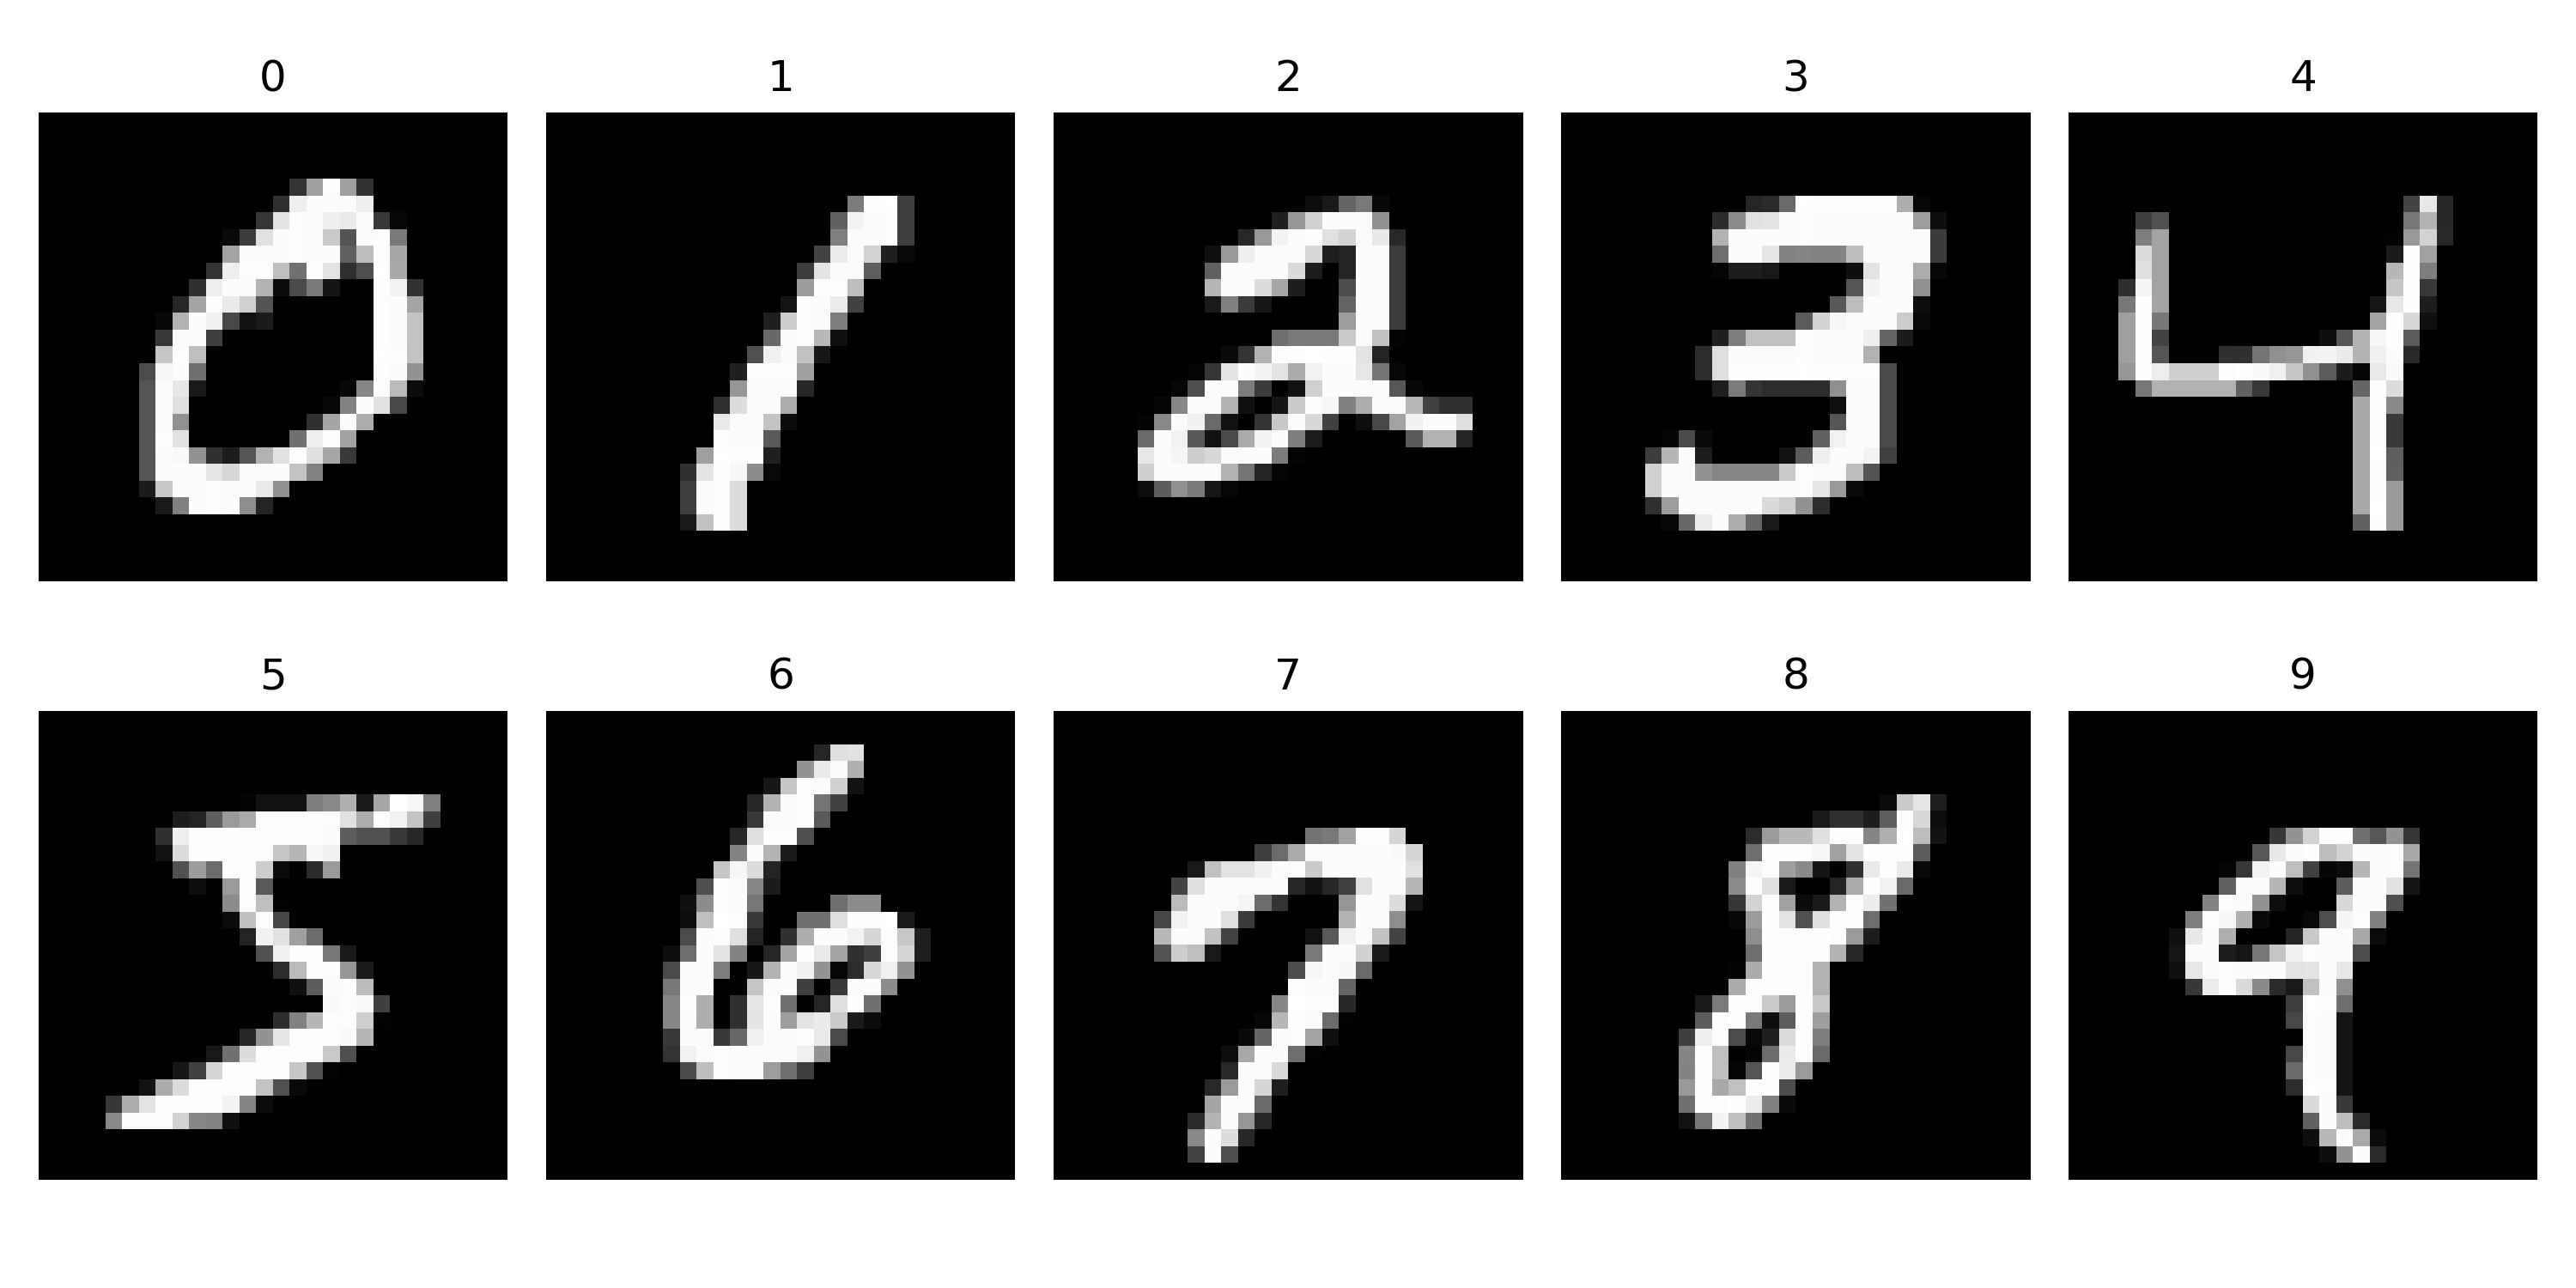
\includegraphics[width=0.48\textwidth]{MNIST_dataset.png}
	\caption{MNIST Dataset \cite{deng2012mnist}}
	\label{fig:mnist_dataset}
\end{figure}
The MNIST dataset is a widely used collection of handwritten digits that is commonly used for training and testing machine learning and computer vision algorithms. MNIST stands for the "Modified National Institute of Standards and Technology" database. It was created by modifying the original NIST dataset, which contained a much larger and more diverse set of handwritten characters, to focus specifically on handwritten digits.

The MNIST dataset contains 28x28-pixel grayscale images of handwritten digits (0 through 9), along with corresponding labels indicating which digit each image represents \cite{deng2012mnist}. There are 60,000 training images and 10,000 testing images in the MNIST dataset, making it a popular benchmark for various image classification tasks.
\subsubsection{ConvNet-3}
\subsubsection{Synthetic Dataset using real images}
\begin{figure}[H]
	\centering
	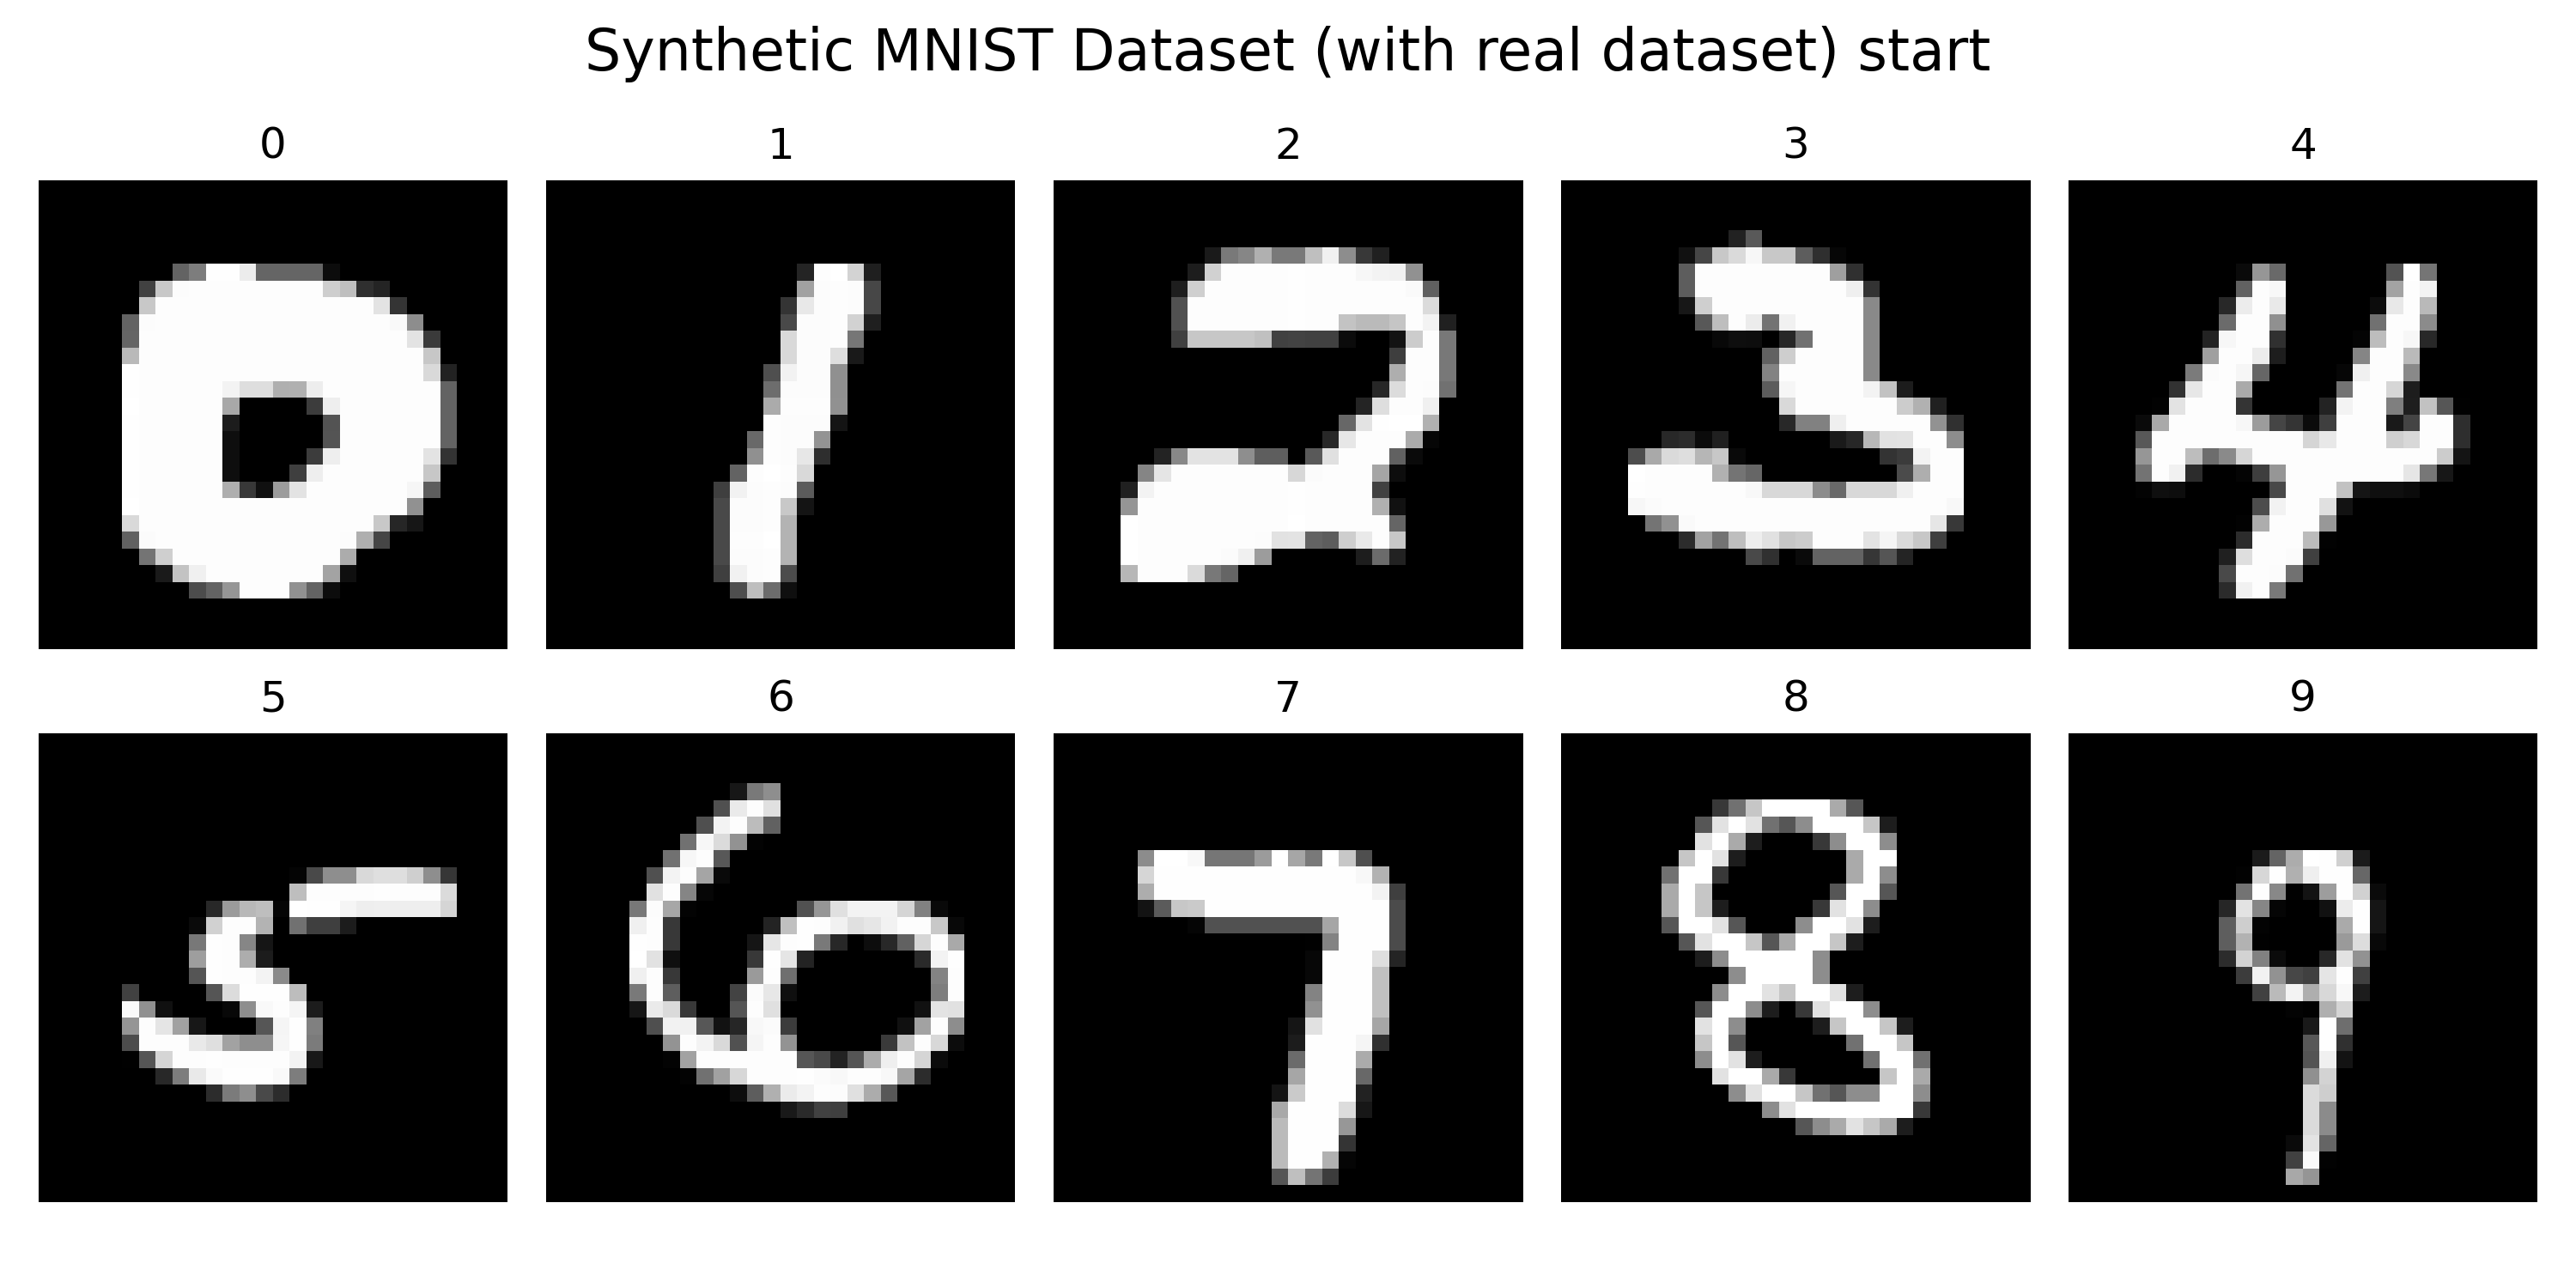
\includegraphics[width=0.48\textwidth]{mnist_real_sample.png}
	\caption{Sample of Synthetic MNIST Dataset created from real images (starting image)}
	\label{fig:mnist_real_sample}
\end{figure}

\begin{figure}[H]
	\centering
	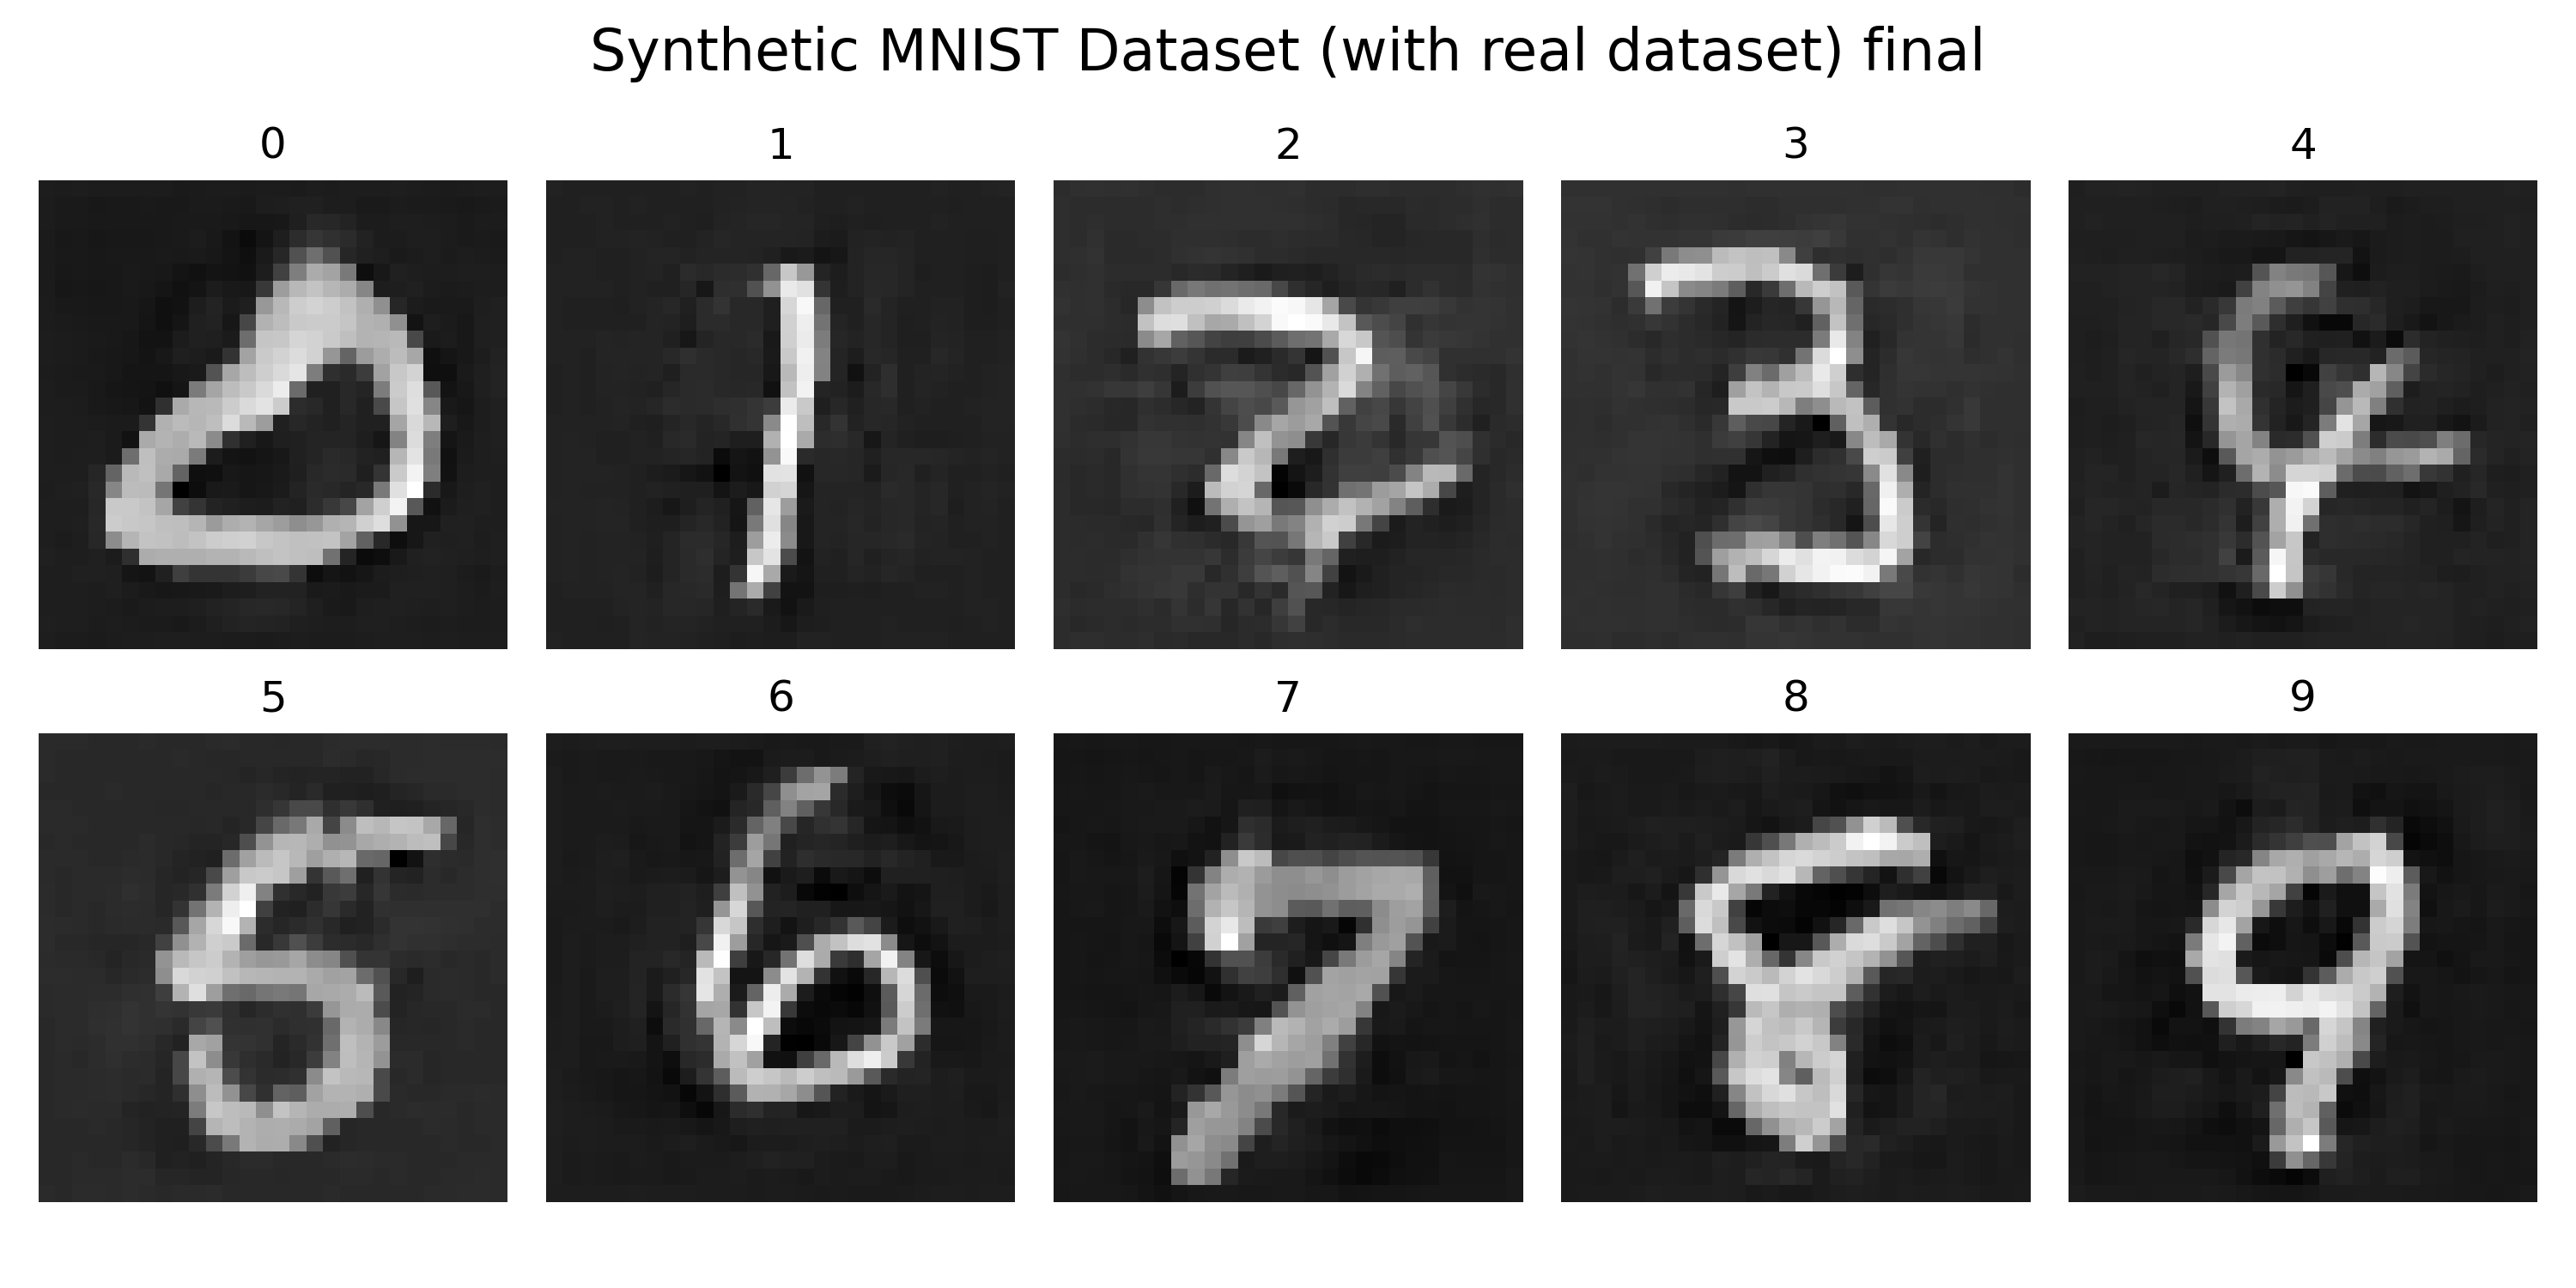
\includegraphics[width=0.48\textwidth]{mnist_real_syn.png}
	\caption{Sample of Synthetic MNIST Dataset created from real images (final image)}
	\label{fig:mnist_real_syn}
\end{figure}

\begin{figure}[H]
	\centering
	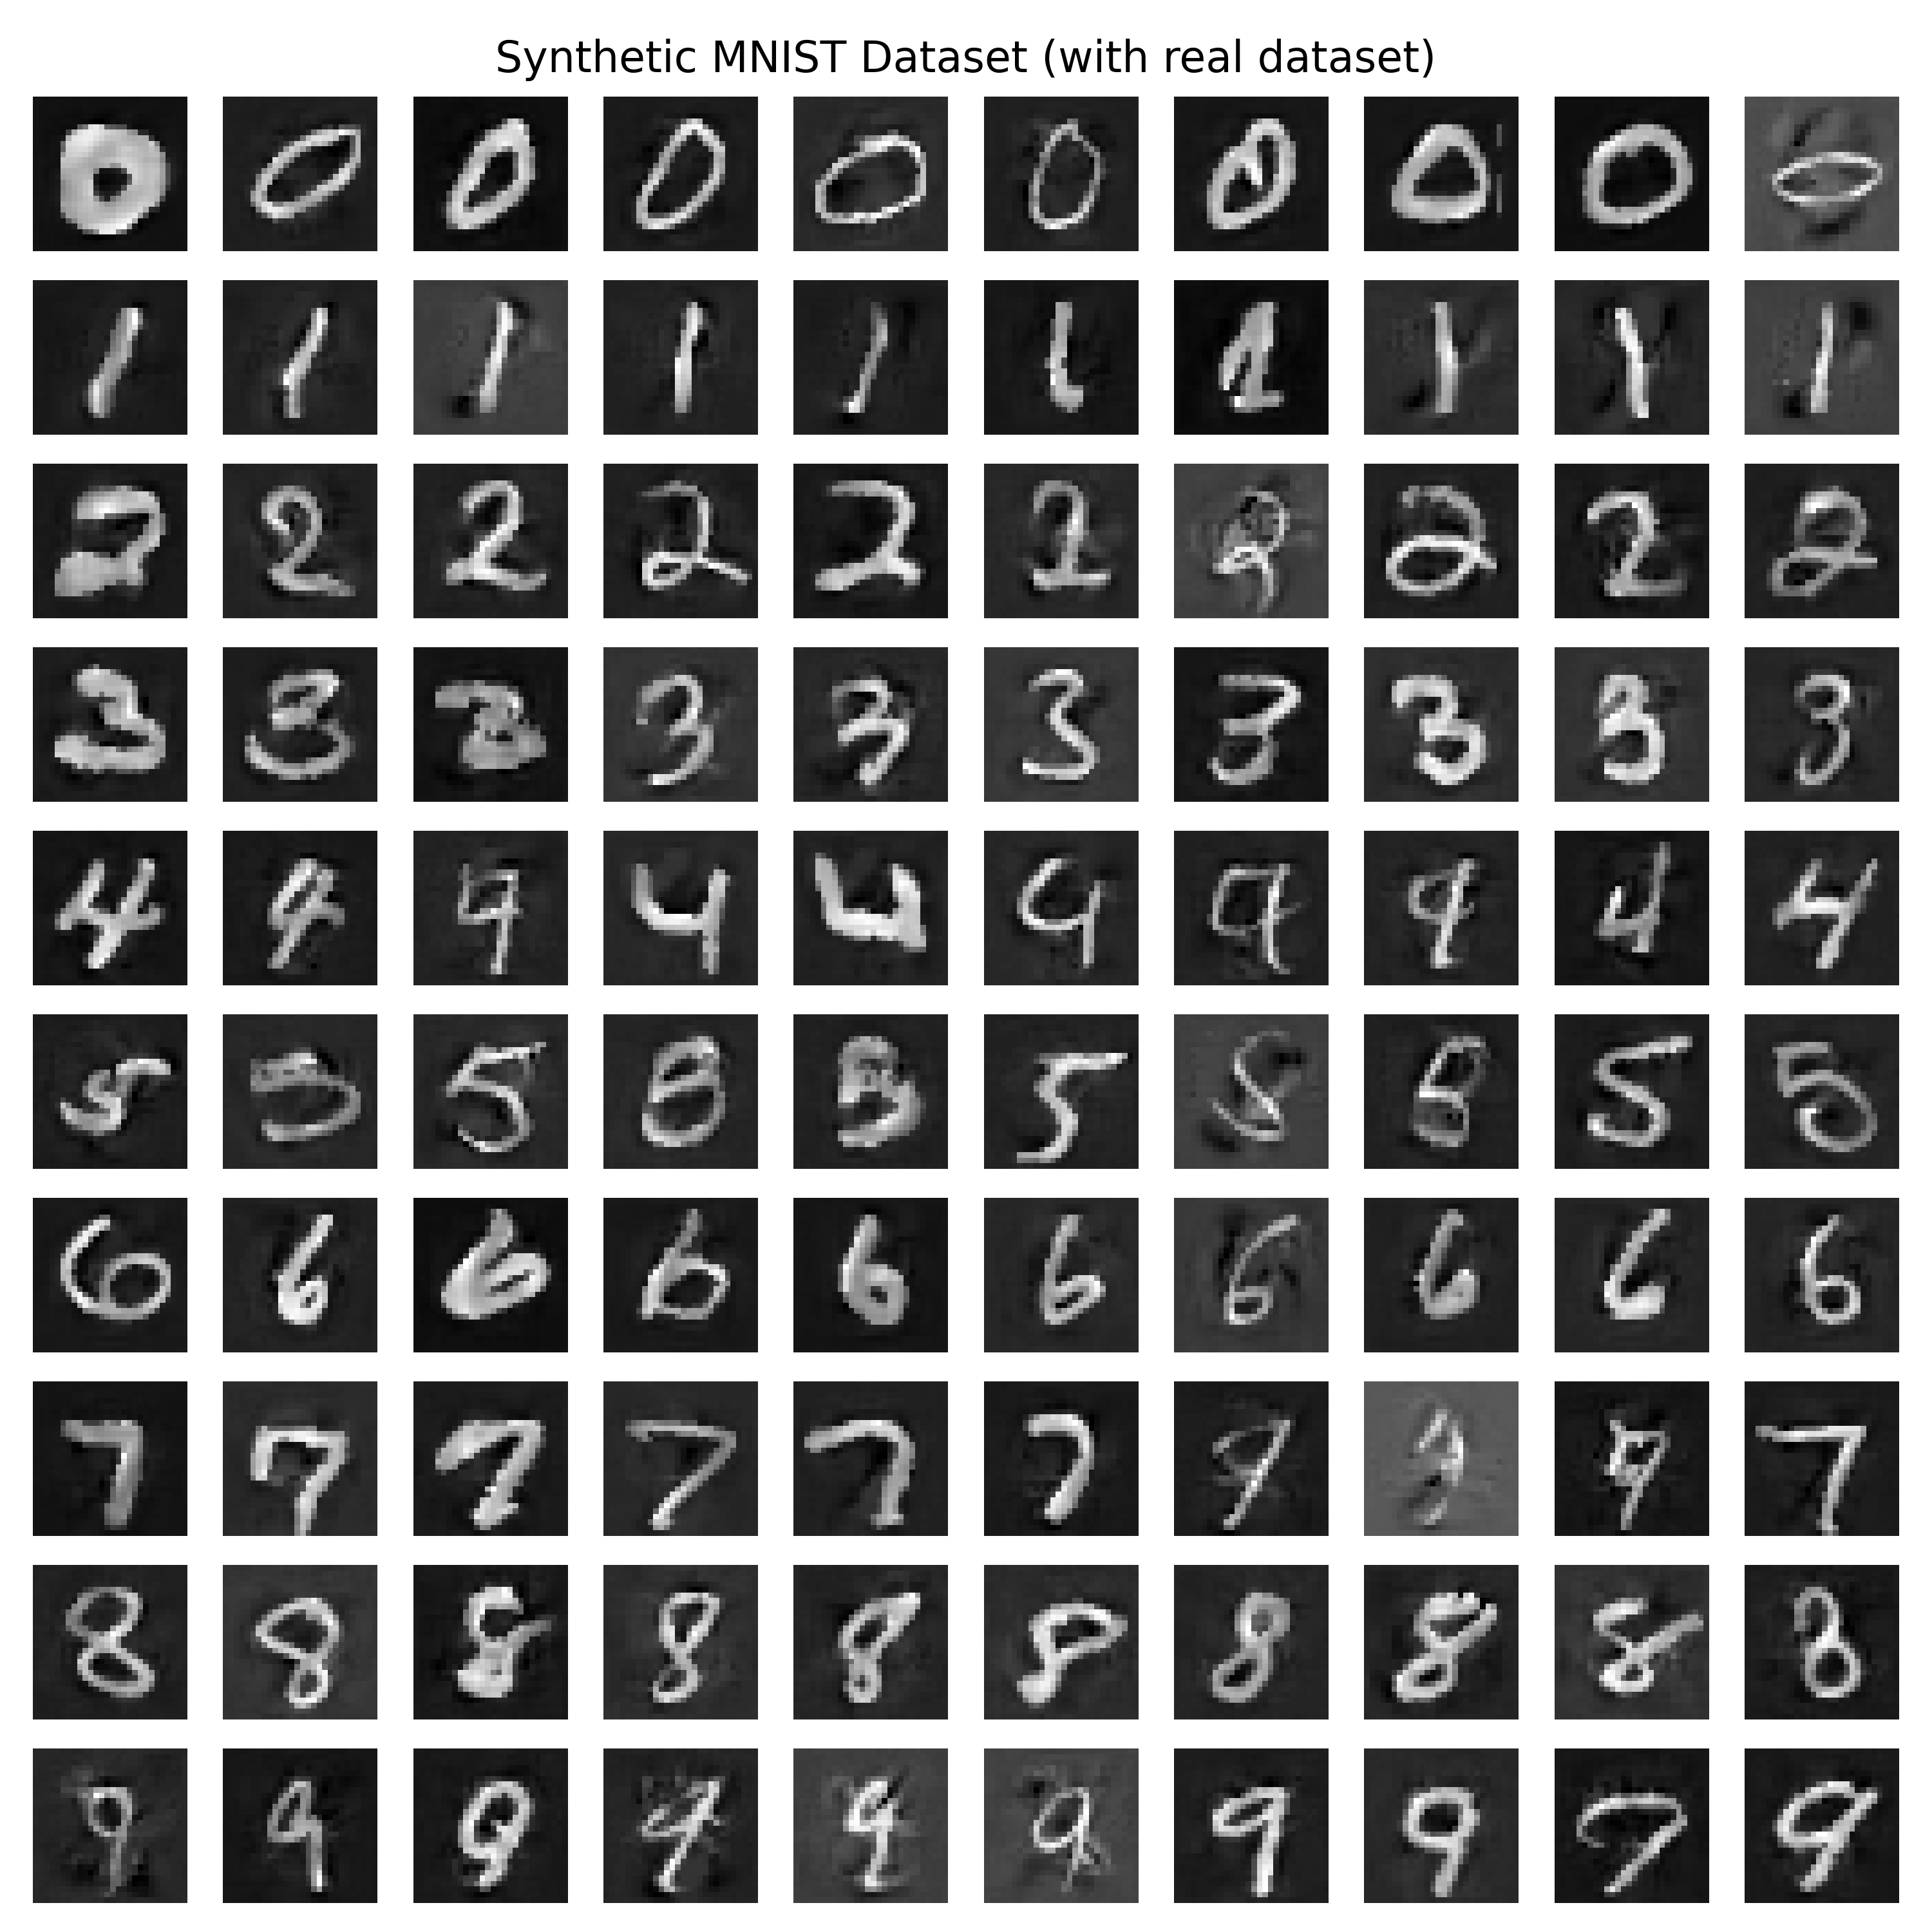
\includegraphics[width=0.48\textwidth]{mnist_real_syn_all.png}
	\caption{Synthetic MNIST Dataset created from real images}
	\label{fig:mnist_real_syn_all}
\end{figure}
\subsubsection{Synthetic Dataset using Gaussian noise}
\begin{figure}[H]
	\centering
	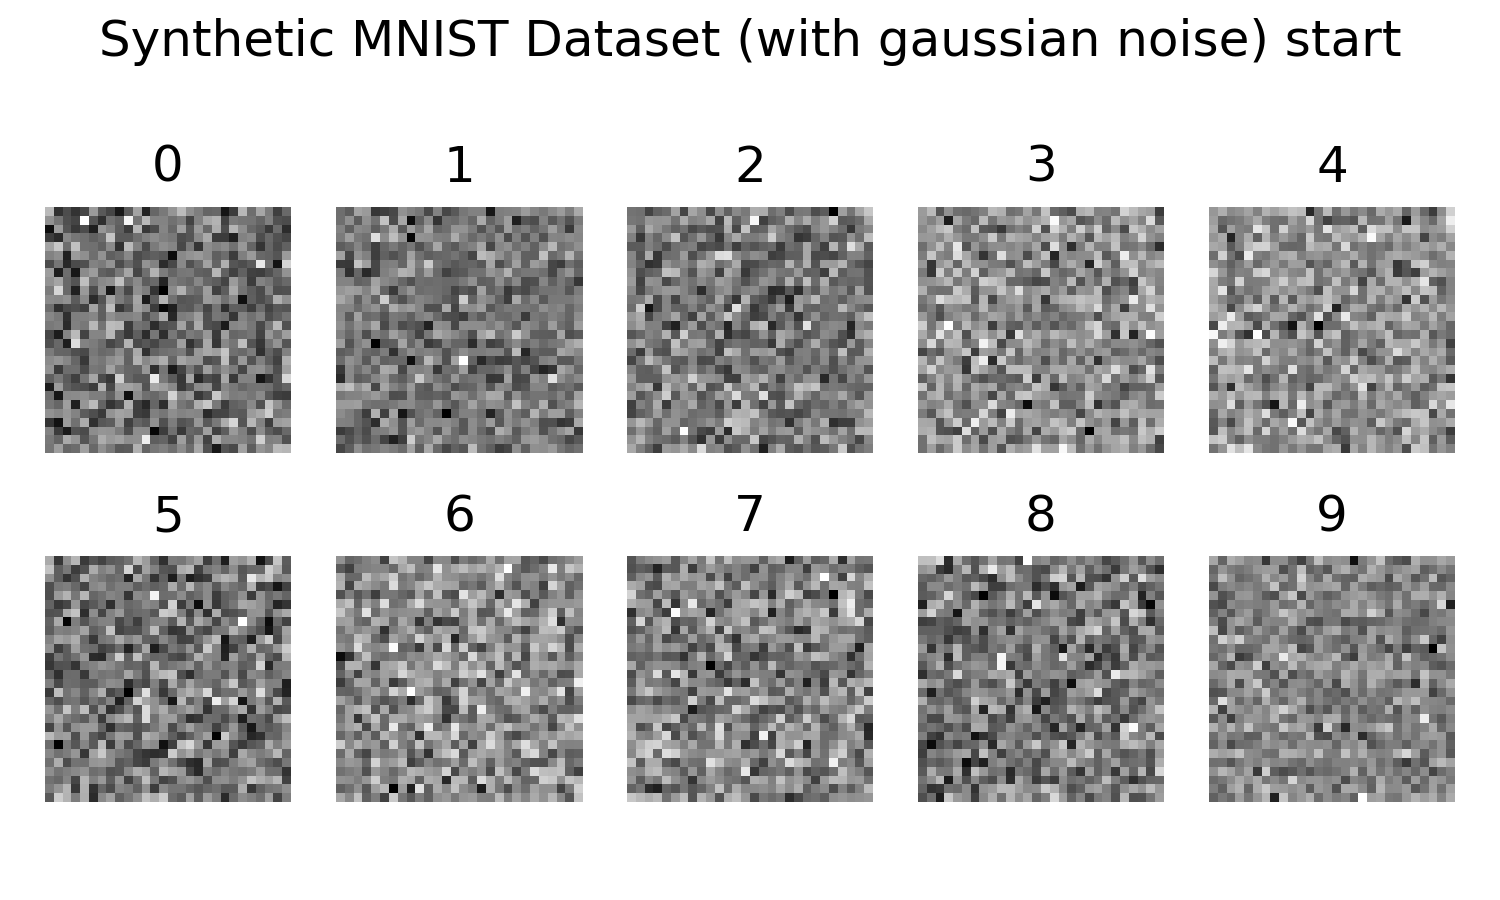
\includegraphics[width=0.48\textwidth]{mnist_noise_sample.png}
	\caption{Sample of Synthetic MNIST Dataset created from Gaussian noise (starting image)}
	\label{fig:mnist_noise_sample}
\end{figure}

\begin{figure}[H]
	\centering
	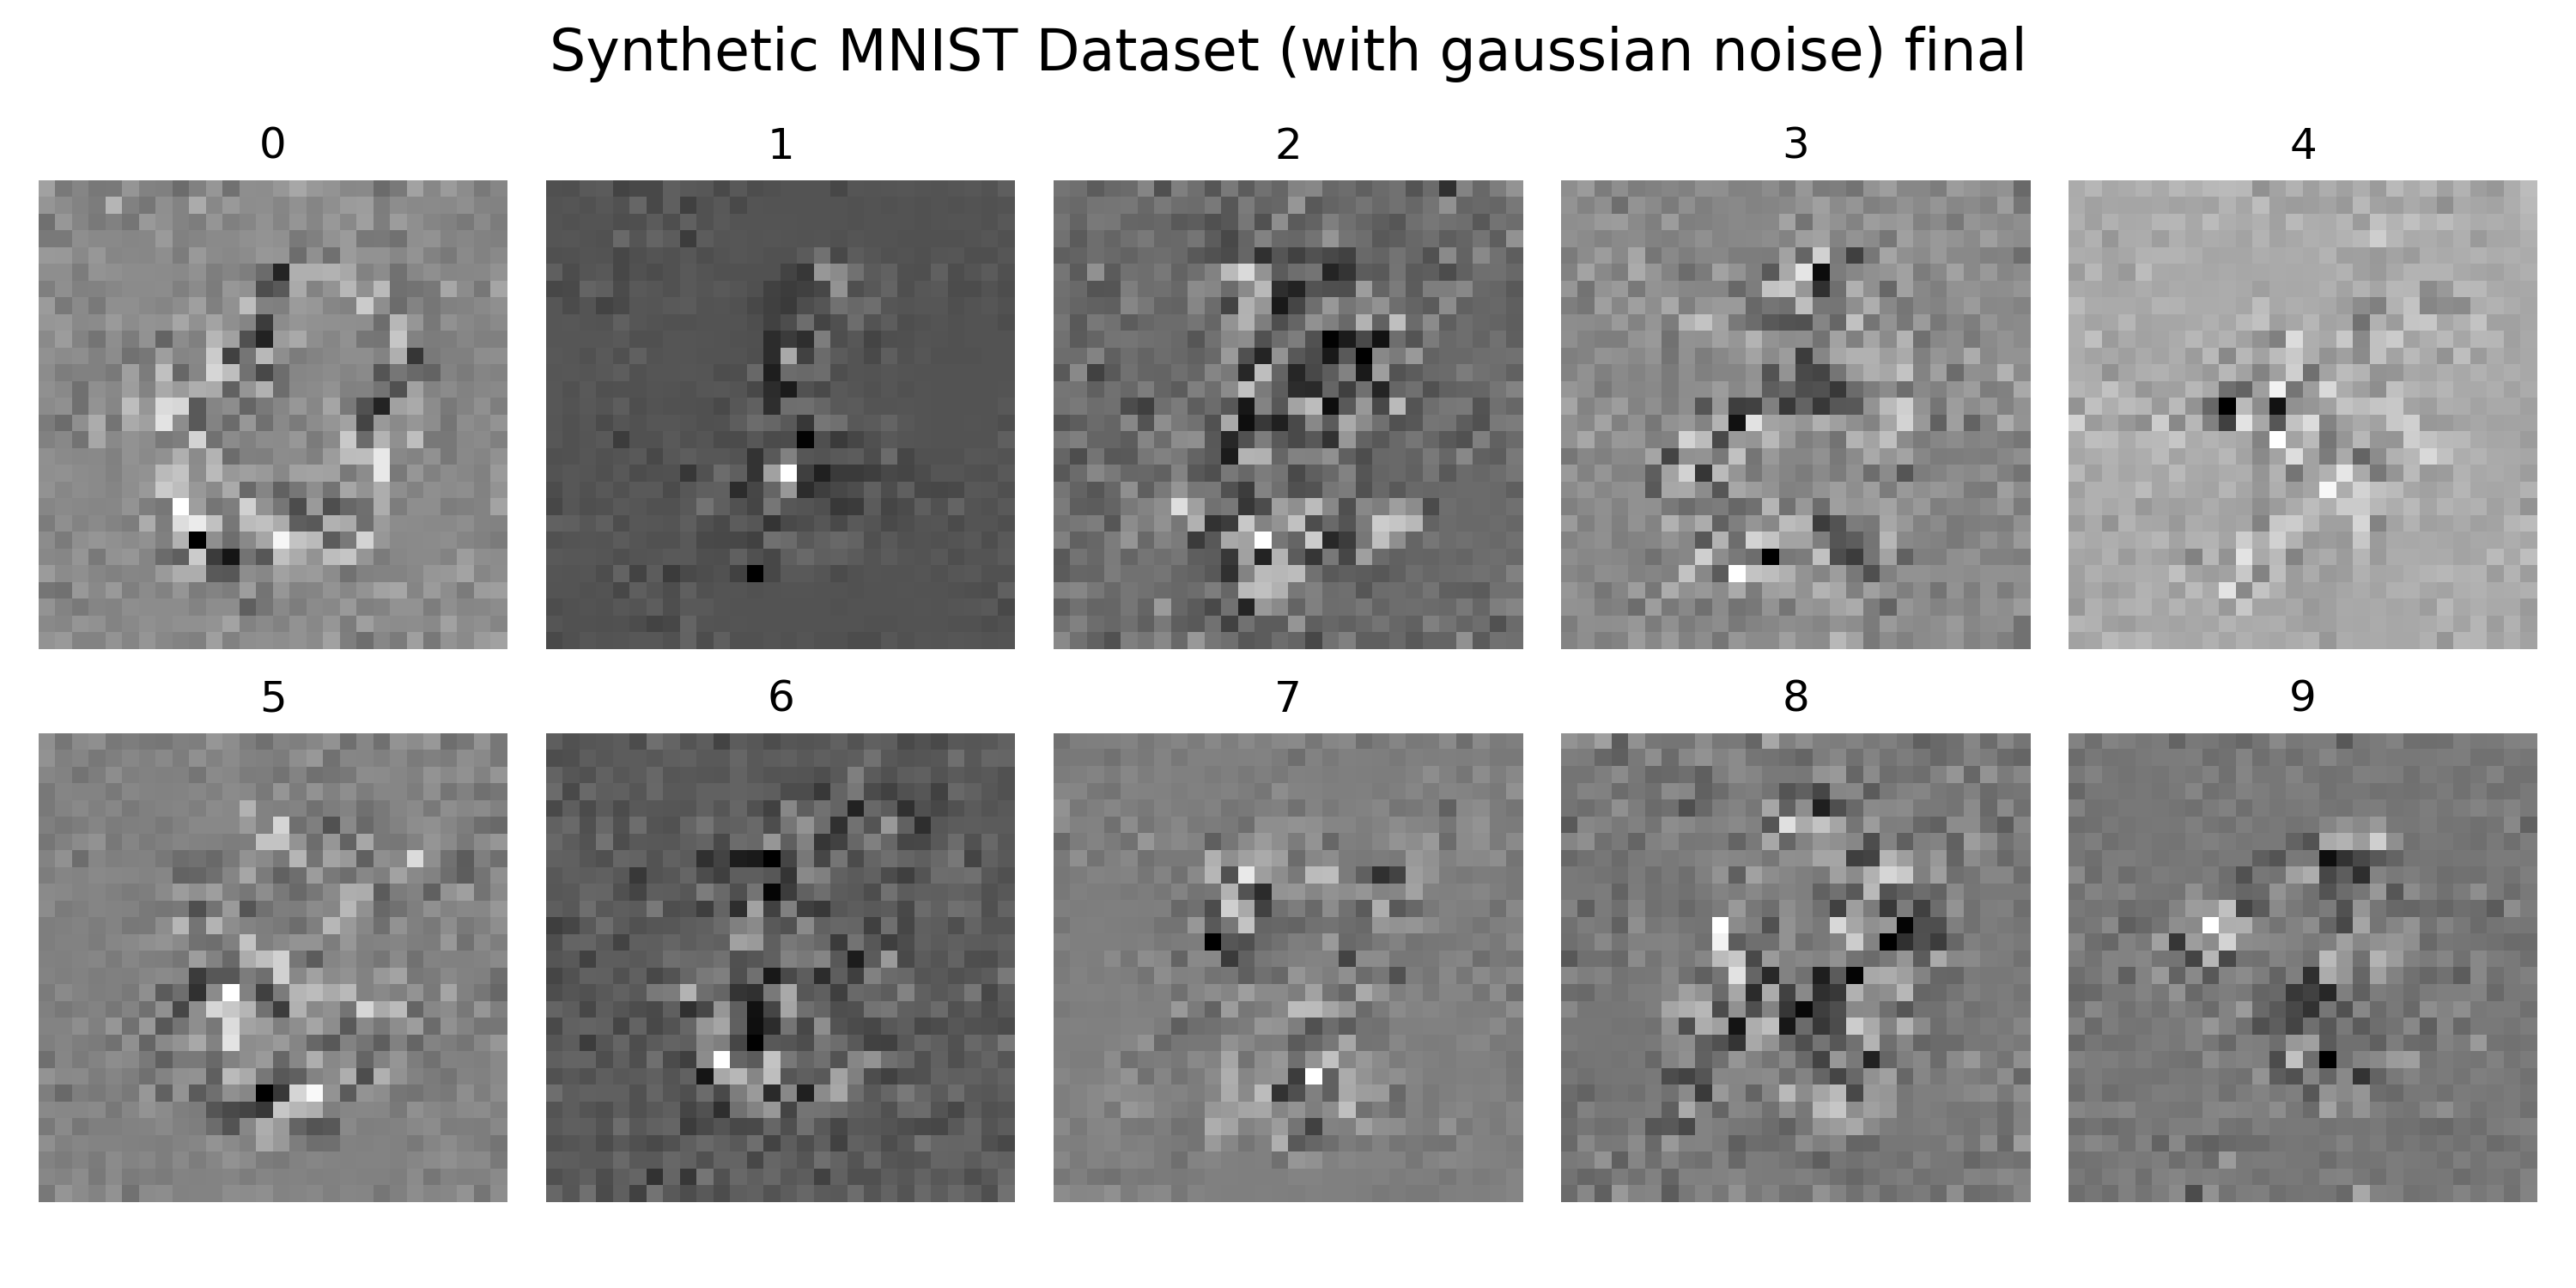
\includegraphics[width=0.48\textwidth]{mnist_noise_syn.png}
	\caption{Sample of Synthetic MNIST Dataset created from Gaussian noise (final image)}
	\label{fig:mnist_noise_syn}
\end{figure}

\begin{figure}[H]
	\centering
	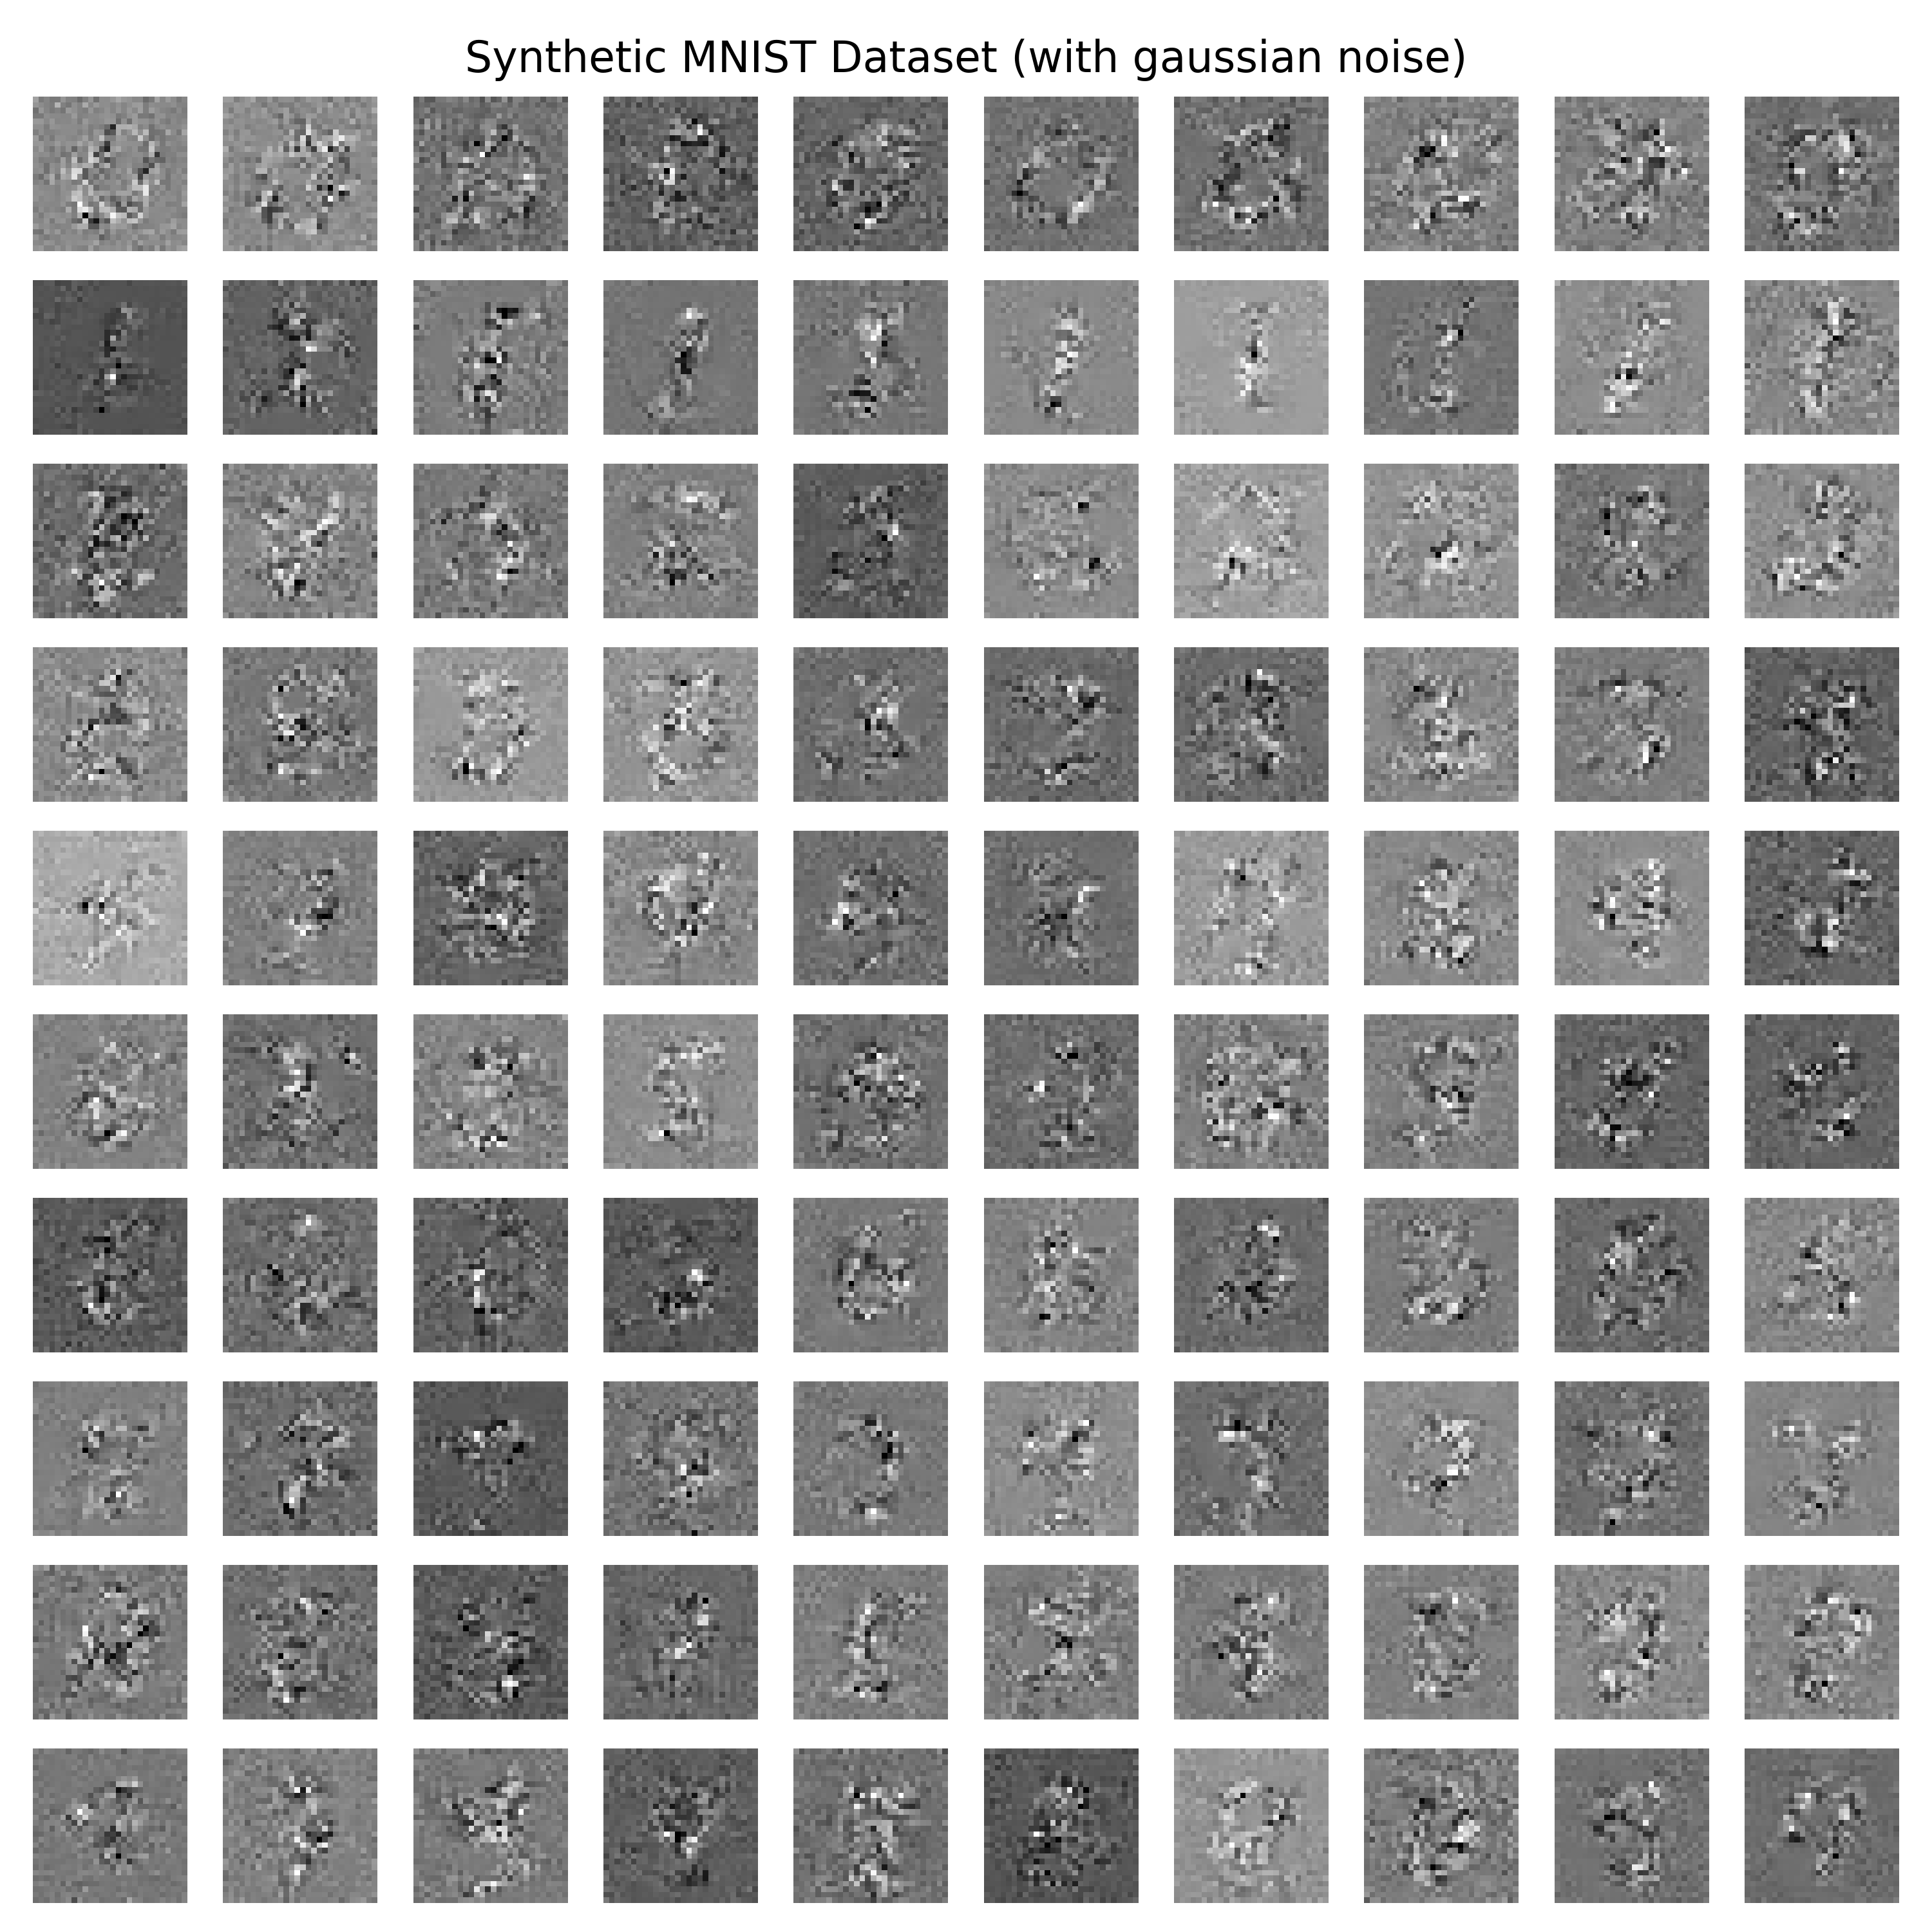
\includegraphics[width=0.48\textwidth]{mnist_noise_syn_all.png}
	\caption{Synthetic MNIST Dataset created from Gaussian noise}
	\label{fig:mnist_noise_syn_all}
\end{figure}
\subsubsection{ConvNet-3 using Synthetic Dataset}
\begin{figure}[H]
	\centering
	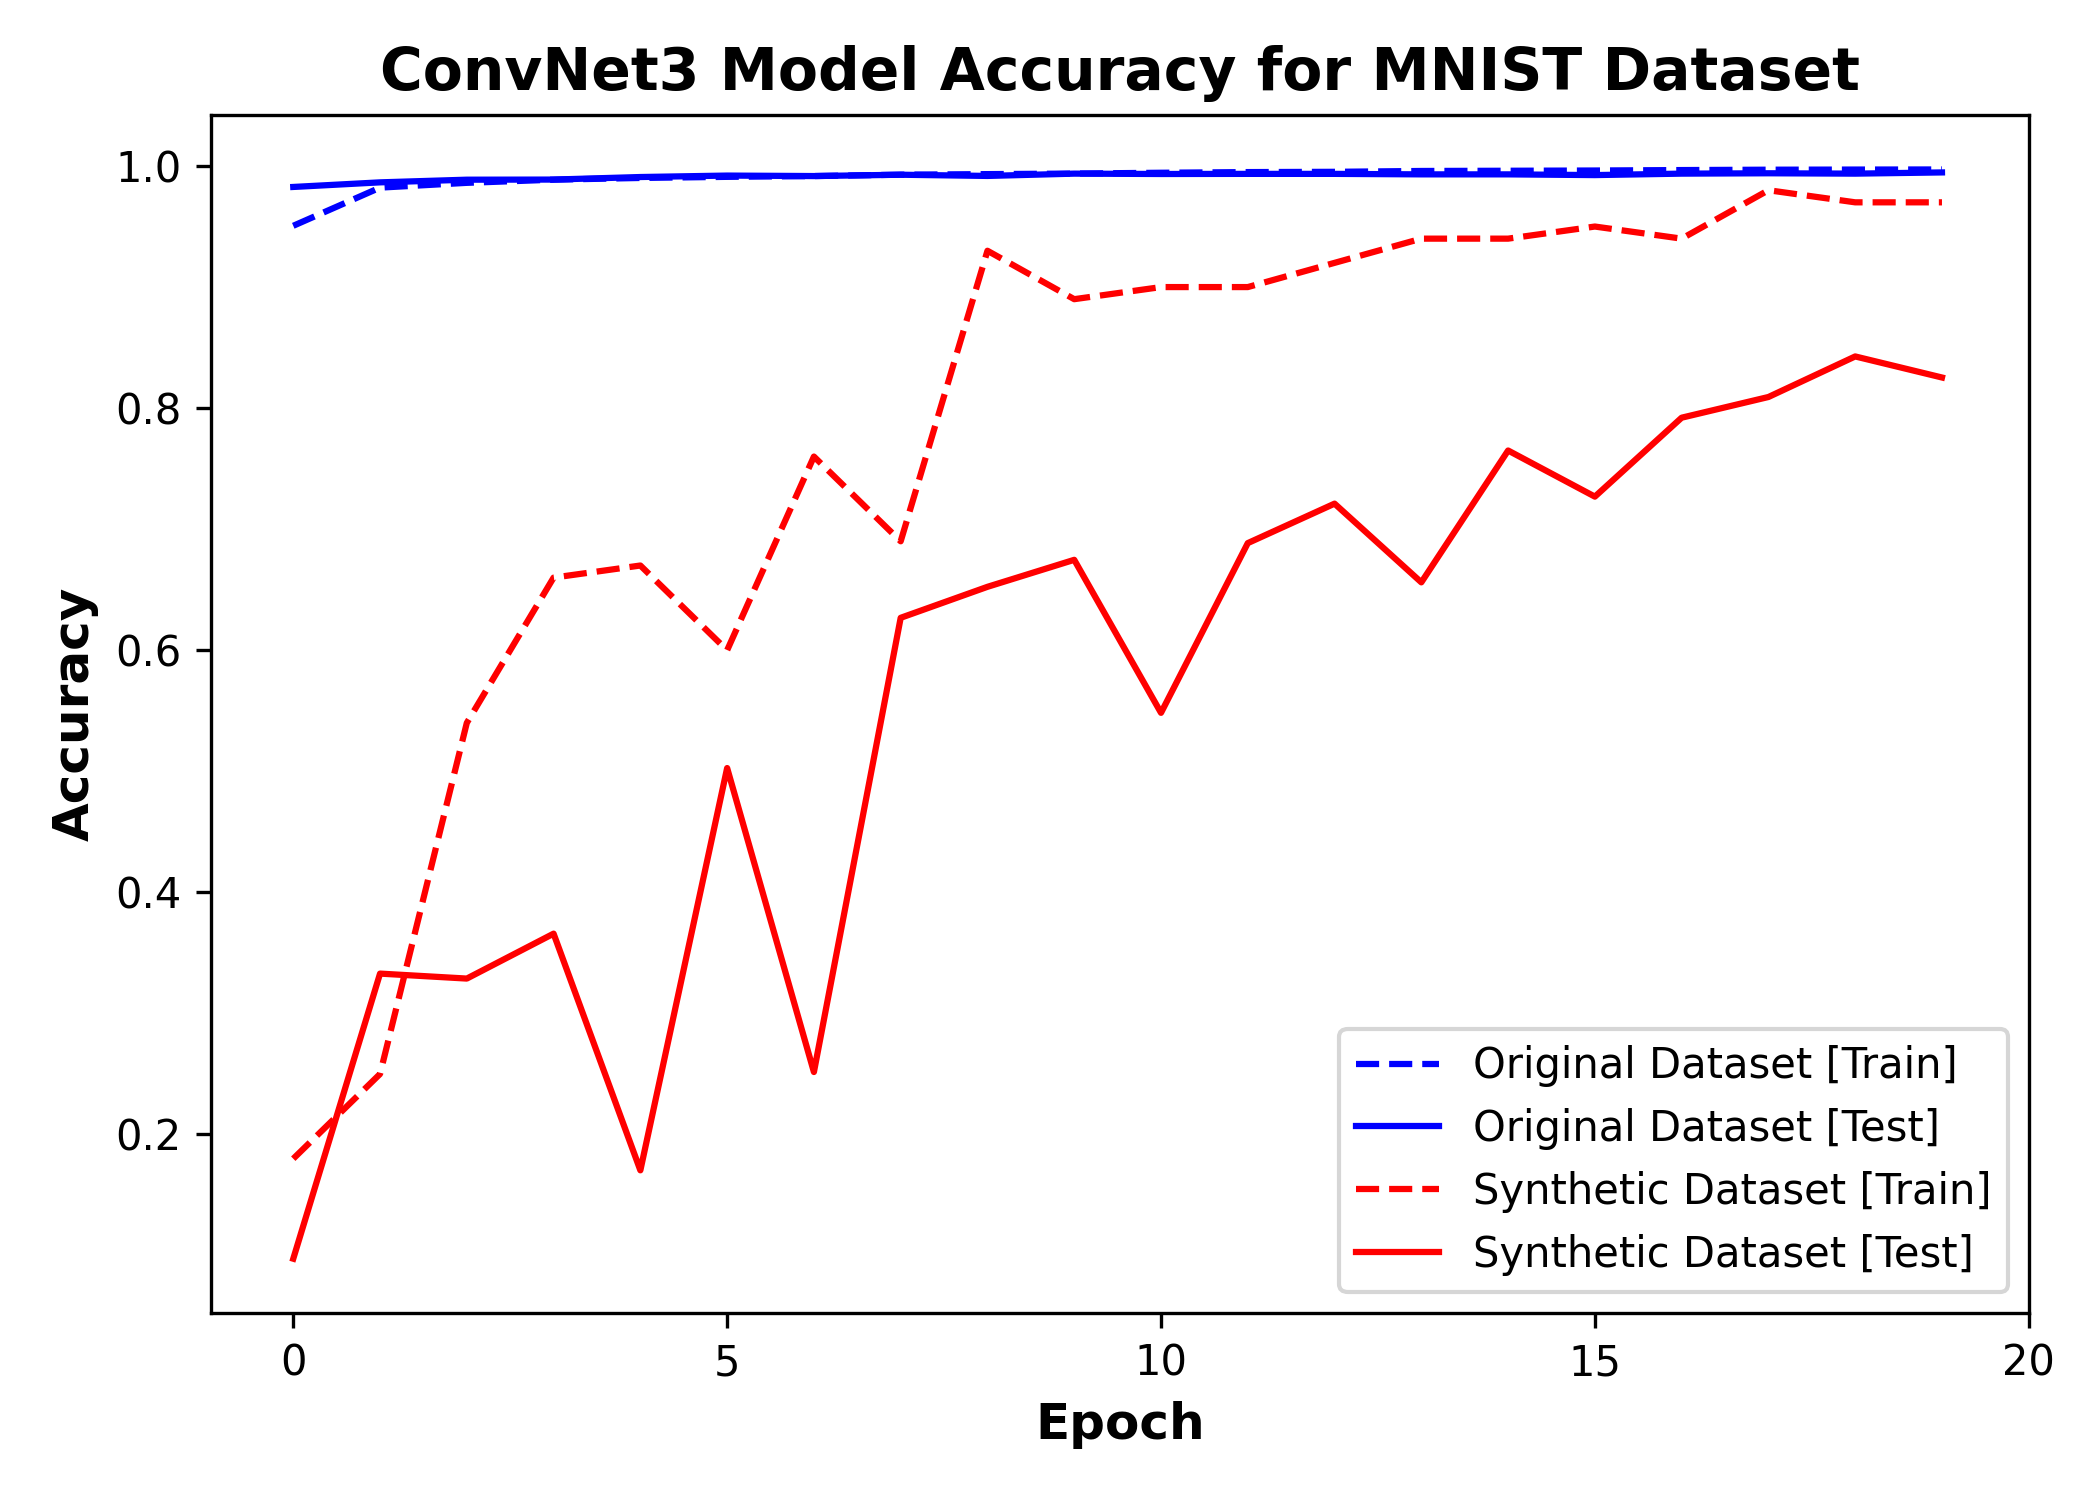
\includegraphics[width=0.48\textwidth]{mnist_syn_acc.png}
	\caption{ConvNet-3 Model Trained using Original and Synthetic dataset}
	\label{fig:mnist_syn_acc}
\end{figure}
\subsubsection{Cross-architecture Generalization - AlexNet}
\begin{figure}[H]
	\centering
	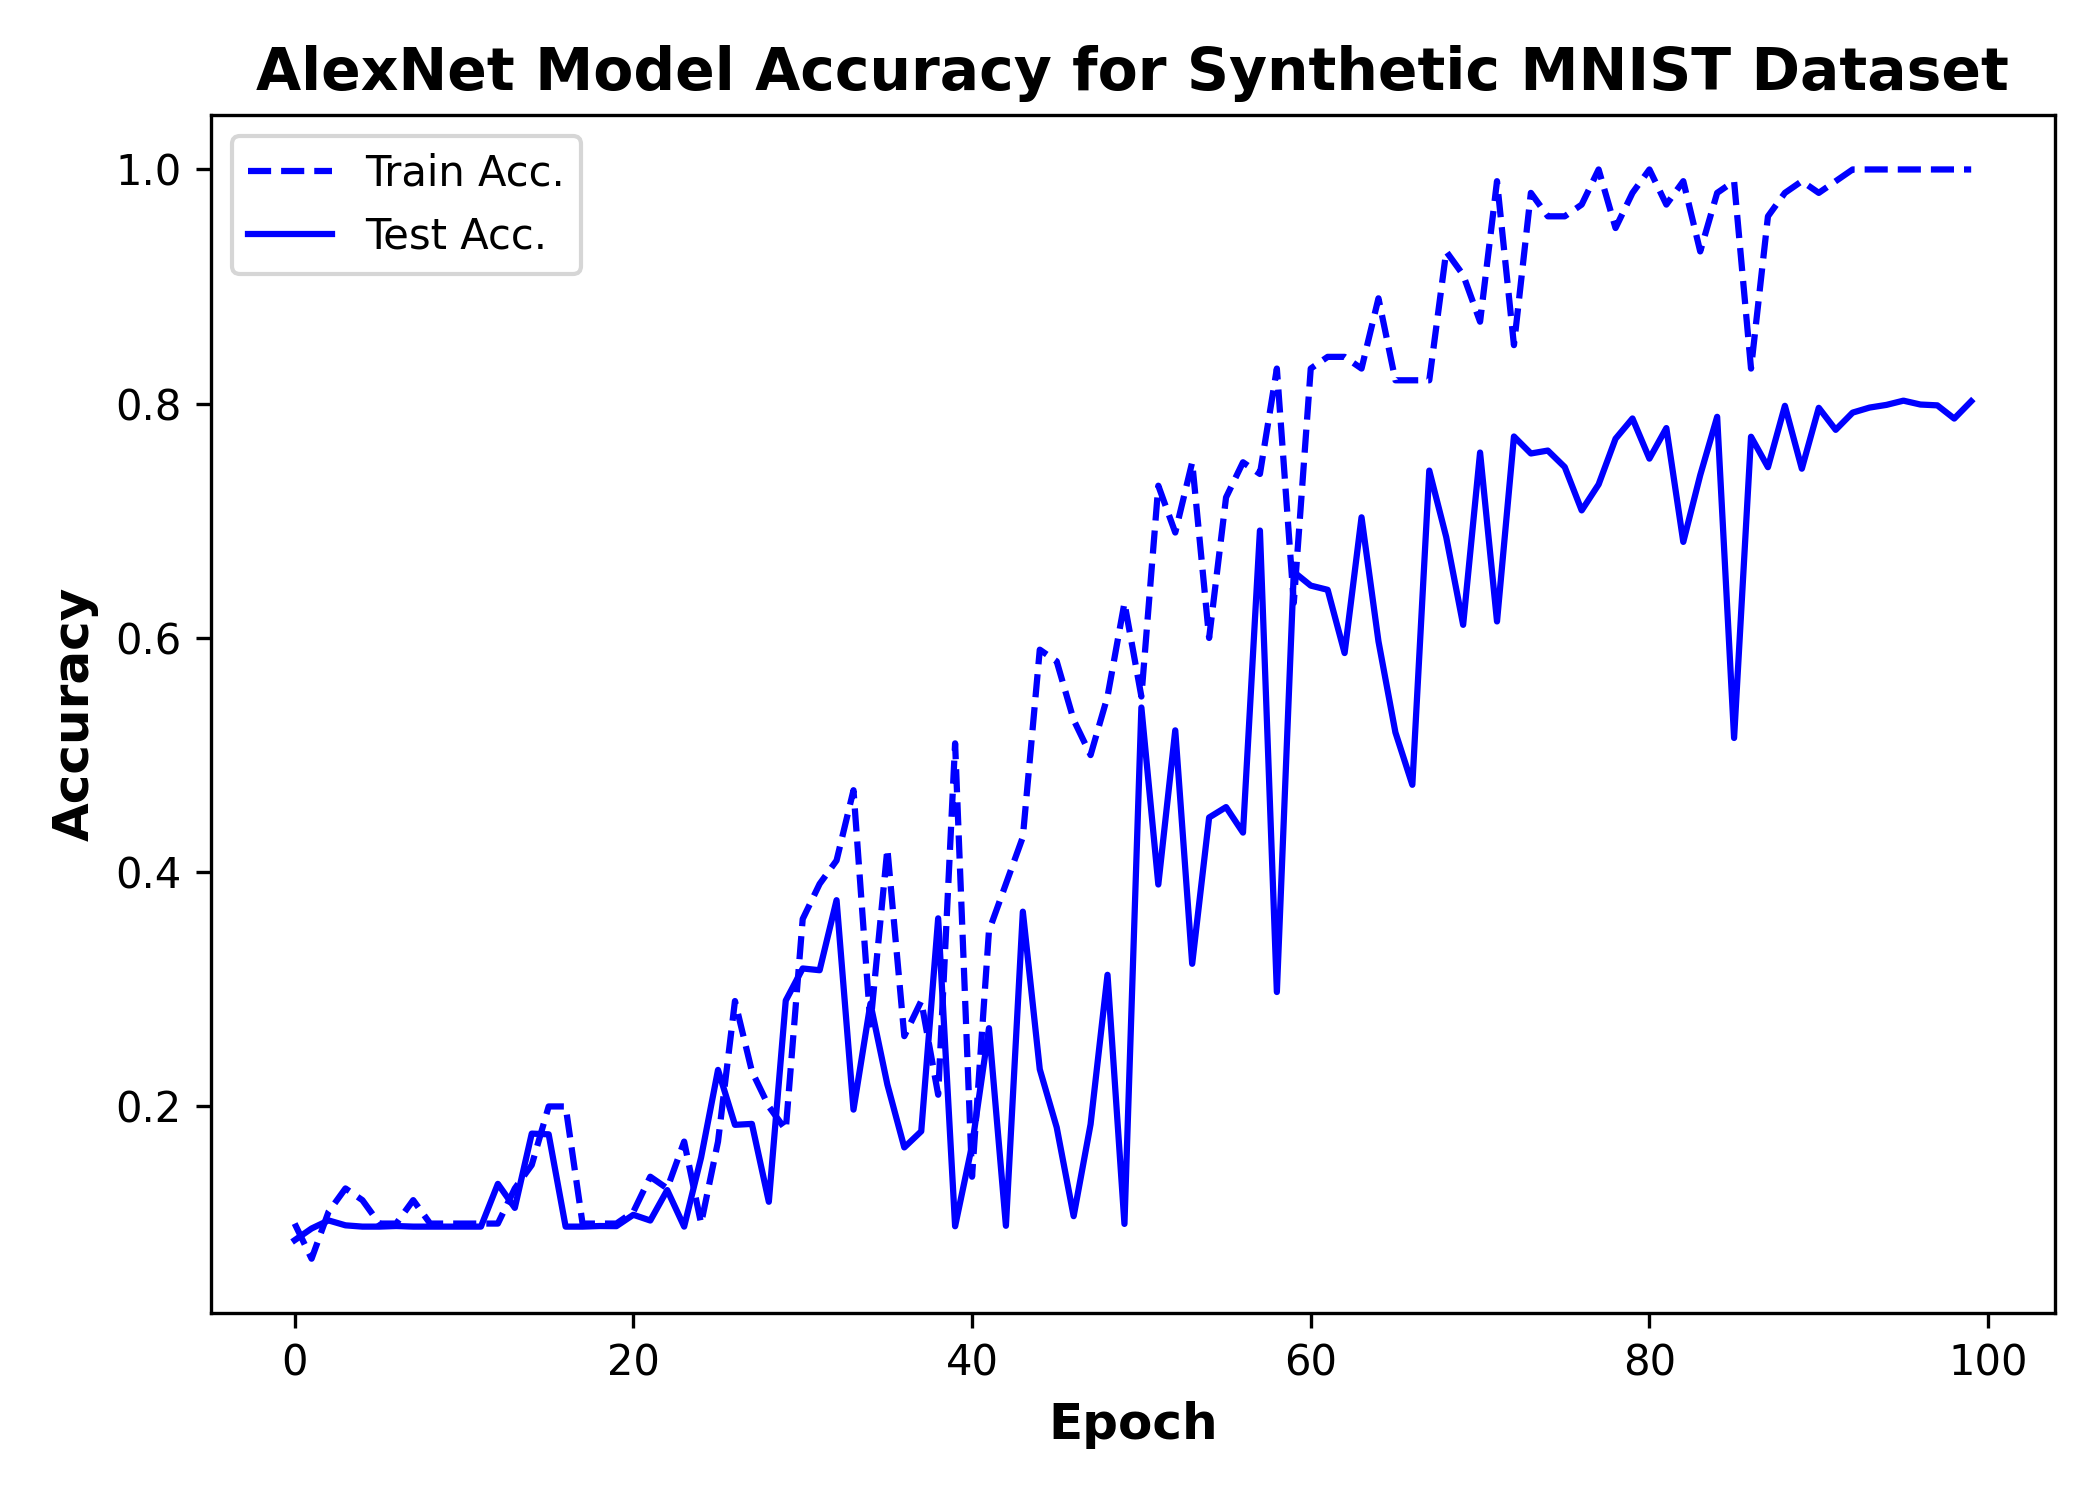
\includegraphics[width=0.48\textwidth]{mnist_alex_acc.png}
	\caption{AlexNet Model Trained using Synthetic dataset}
	\label{fig:mnist_alex_acc}
\end{figure}
\subsection{MHIST Dataset}
\begin{figure}[H]
	\centering
	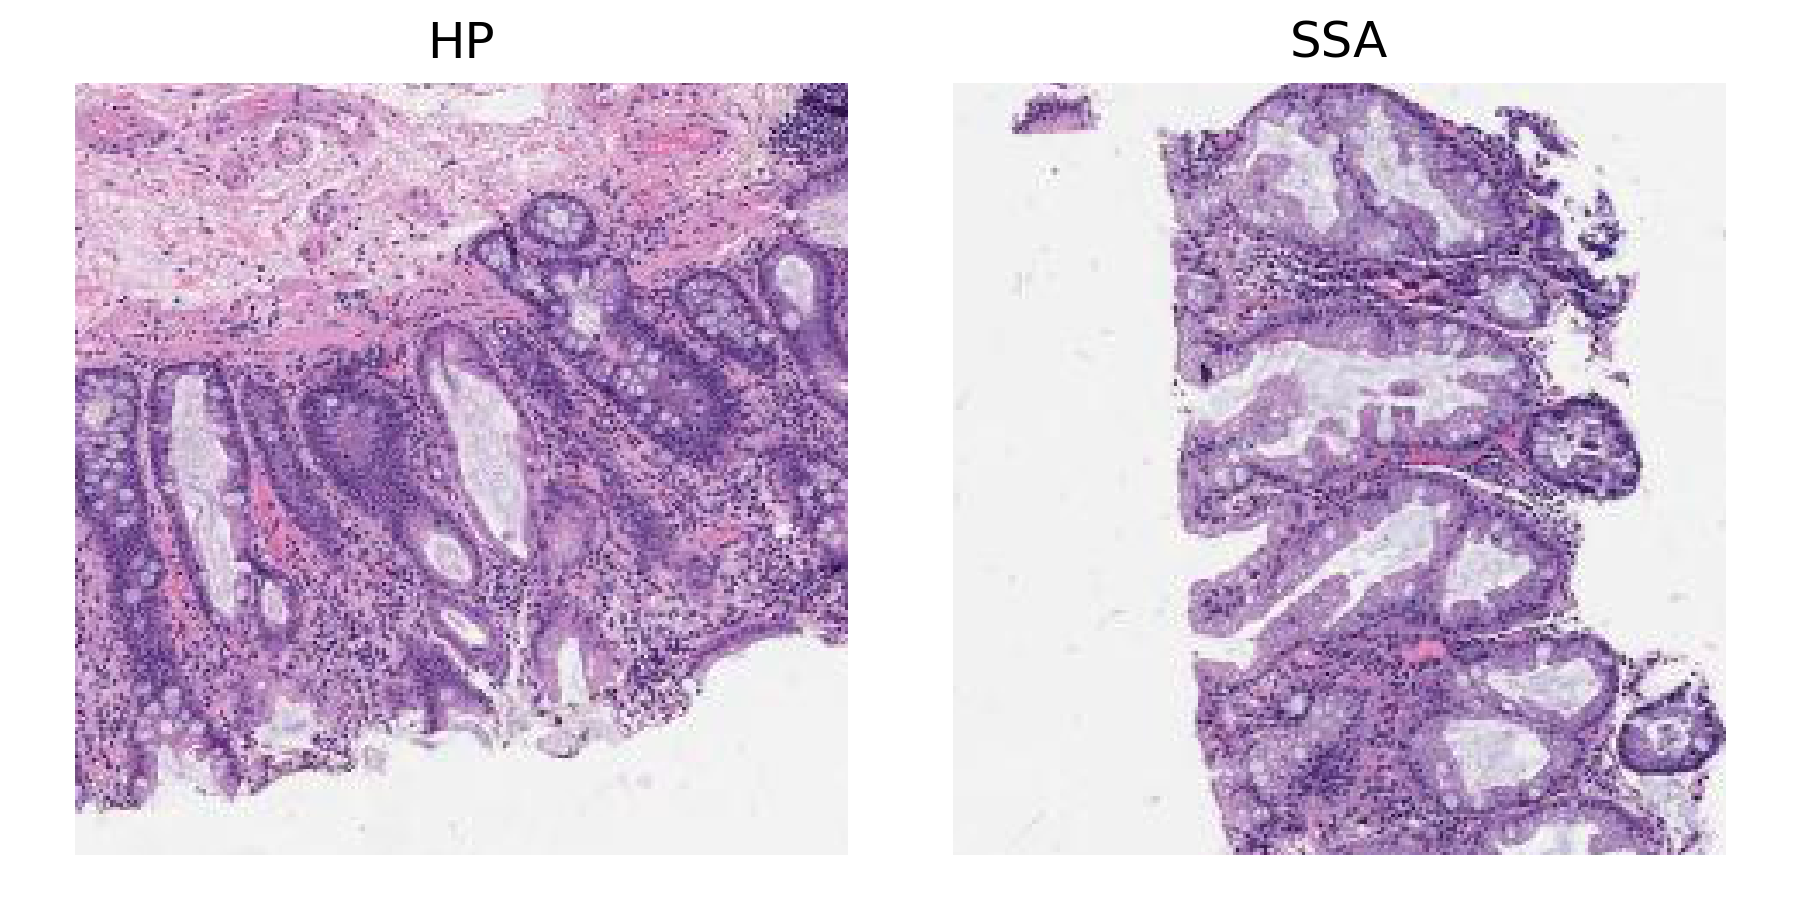
\includegraphics[width=0.48\textwidth]{MHIST_dataset.png}
	\caption{MHIST Dataset \cite{wei2021petri}}
	\label{fig:mhist_dataset}
\end{figure}

\subsubsection{Synthetic Dataset using real images}
\begin{figure}[H]
	\centering
	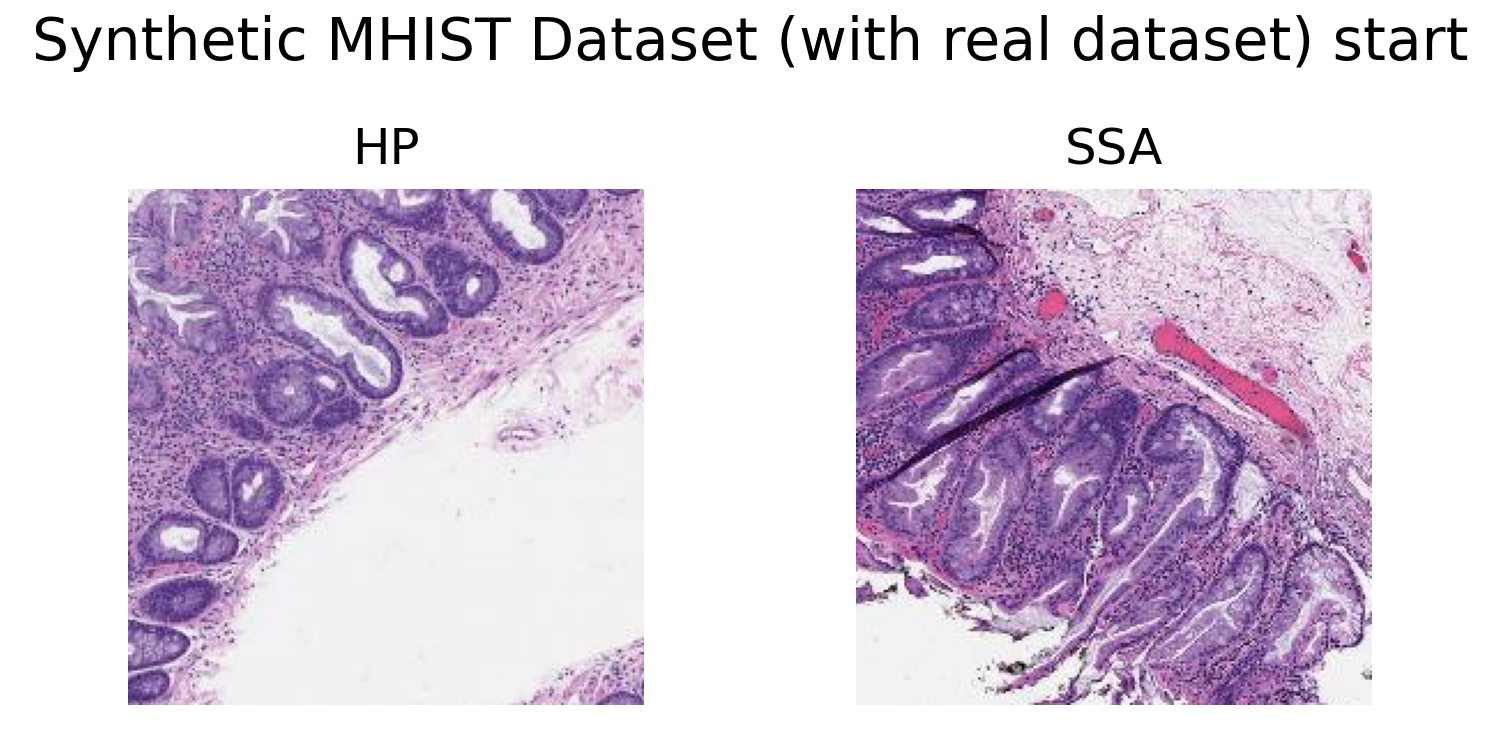
\includegraphics[width=0.48\textwidth]{mhist_real_sample.png}
	\caption{Sample of Synthetic MHIST Dataset created from real images (starting image)}
	\label{fig:mhist_real_sample}
\end{figure}
\begin{figure}[H]
	\centering
	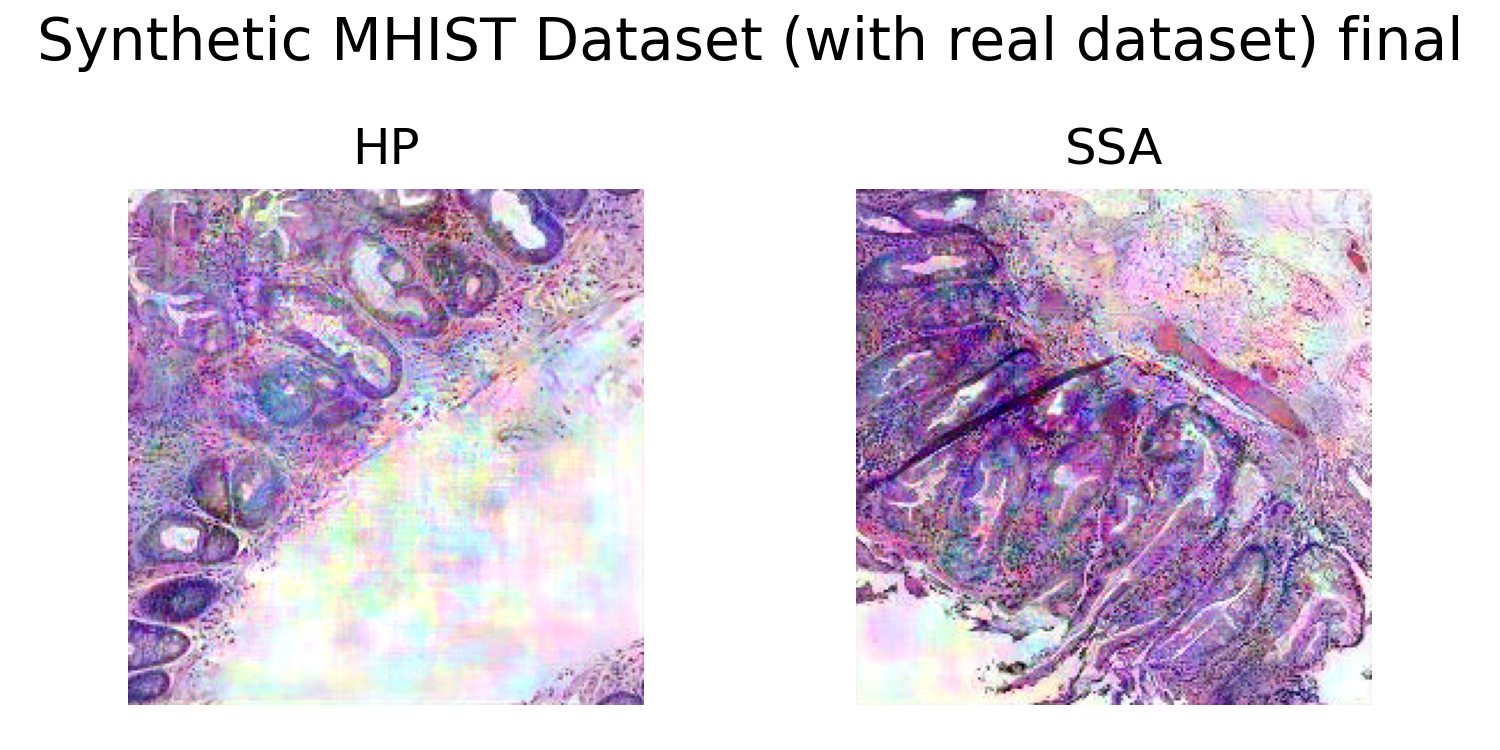
\includegraphics[width=0.48\textwidth]{mhist_real_syn.png}
	\caption{Sample of Synthetic MHIST Dataset created from real images (final image)}
	\label{fig:mhist_real_final}
\end{figure}


\begin{figure}[H]
	\centering
	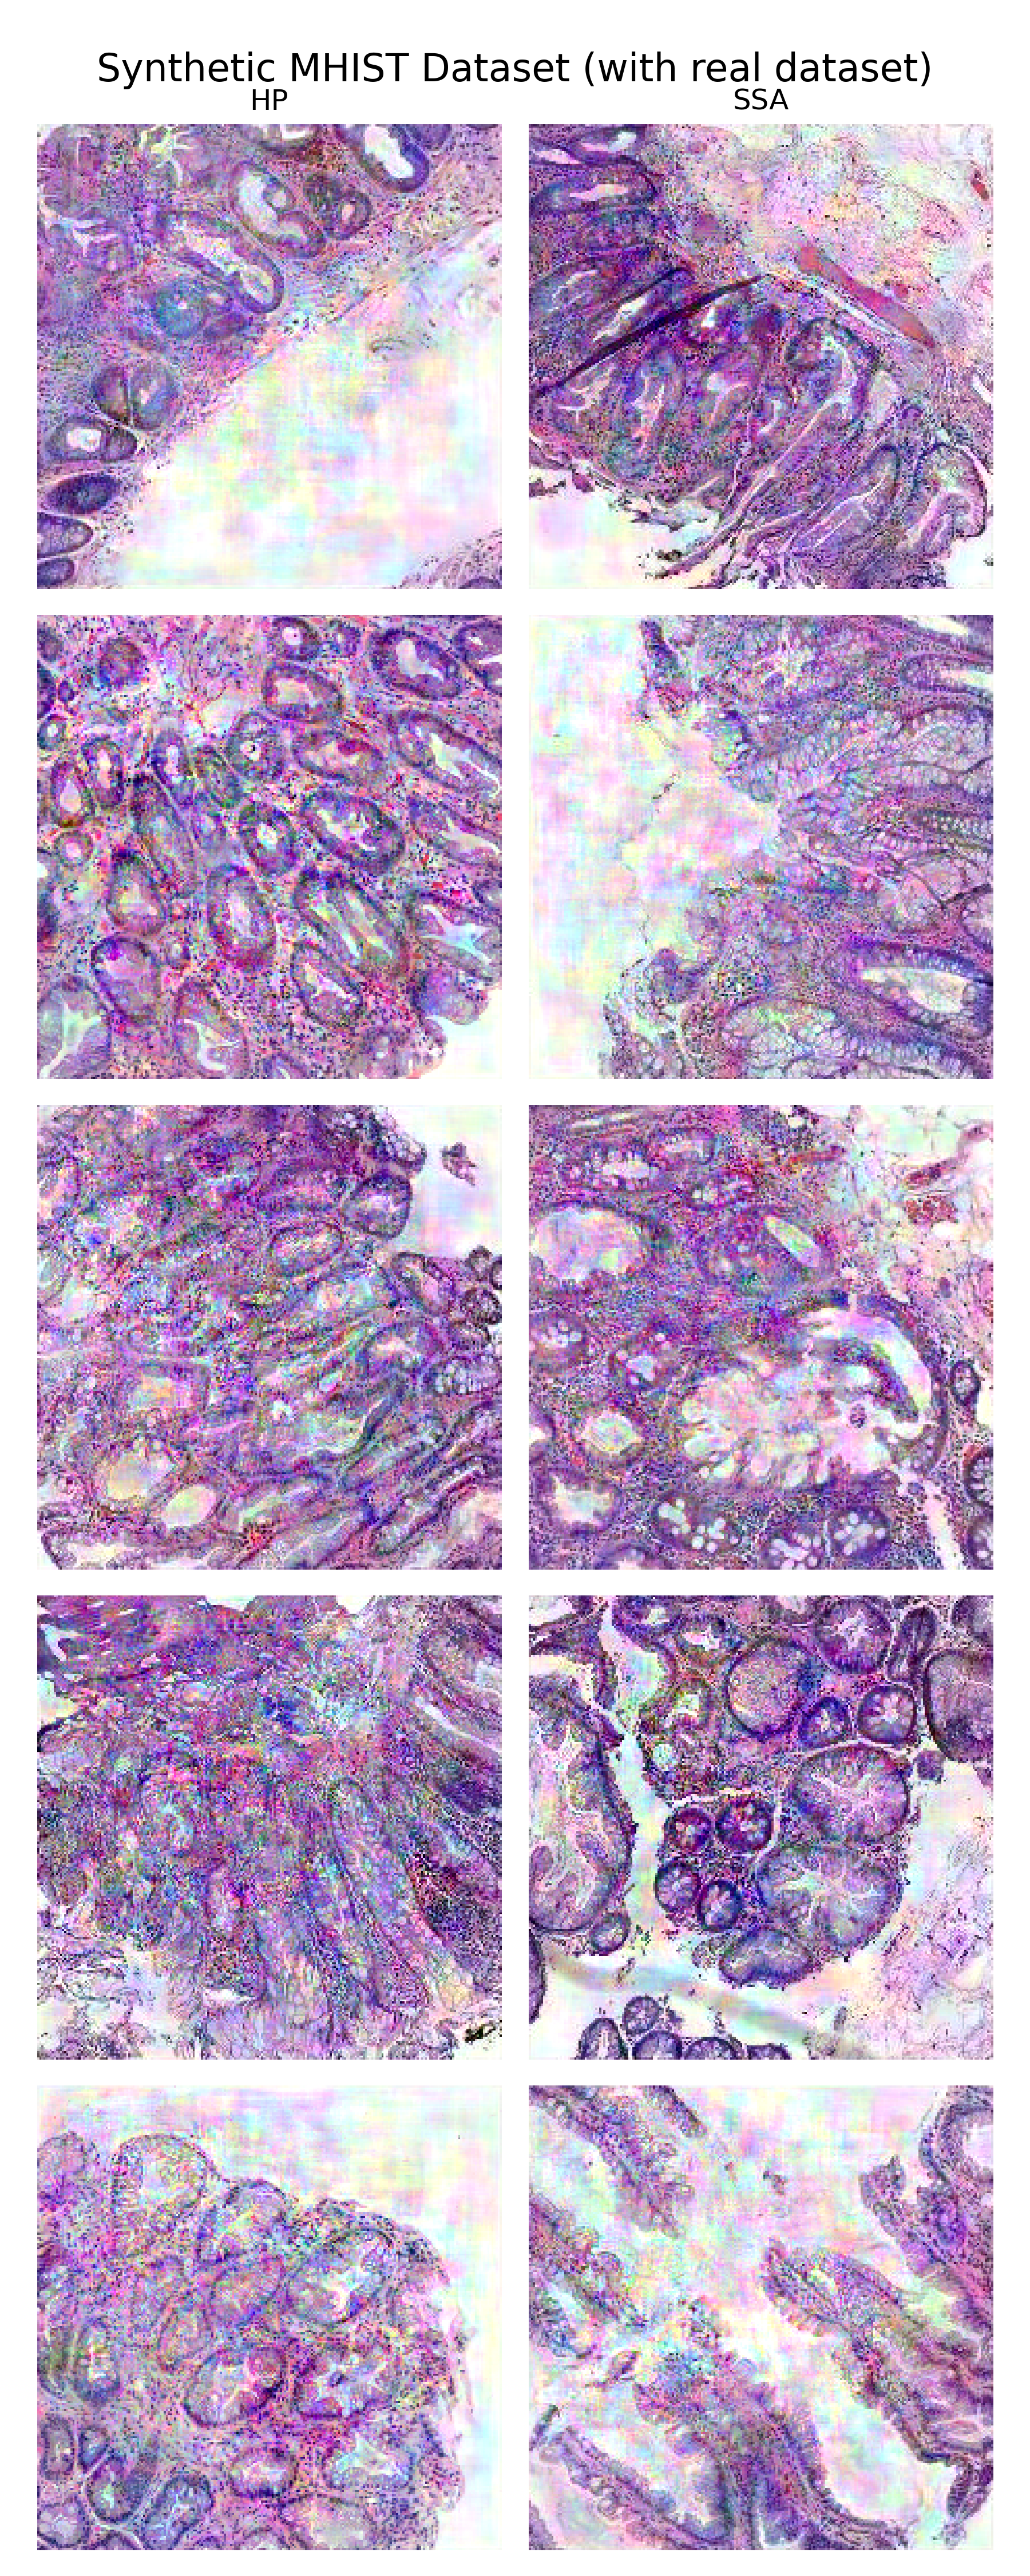
\includegraphics[width=0.48\textwidth]{mhist_real_syn_all.png}
	\caption{Synthetic MHIST Dataset created from real images}
	\label{fig:mhist_real_syn_all}
\end{figure}
\subsubsection{Synthetic Dataset using Gaussian noise}
\begin{figure}[H]
	\centering
	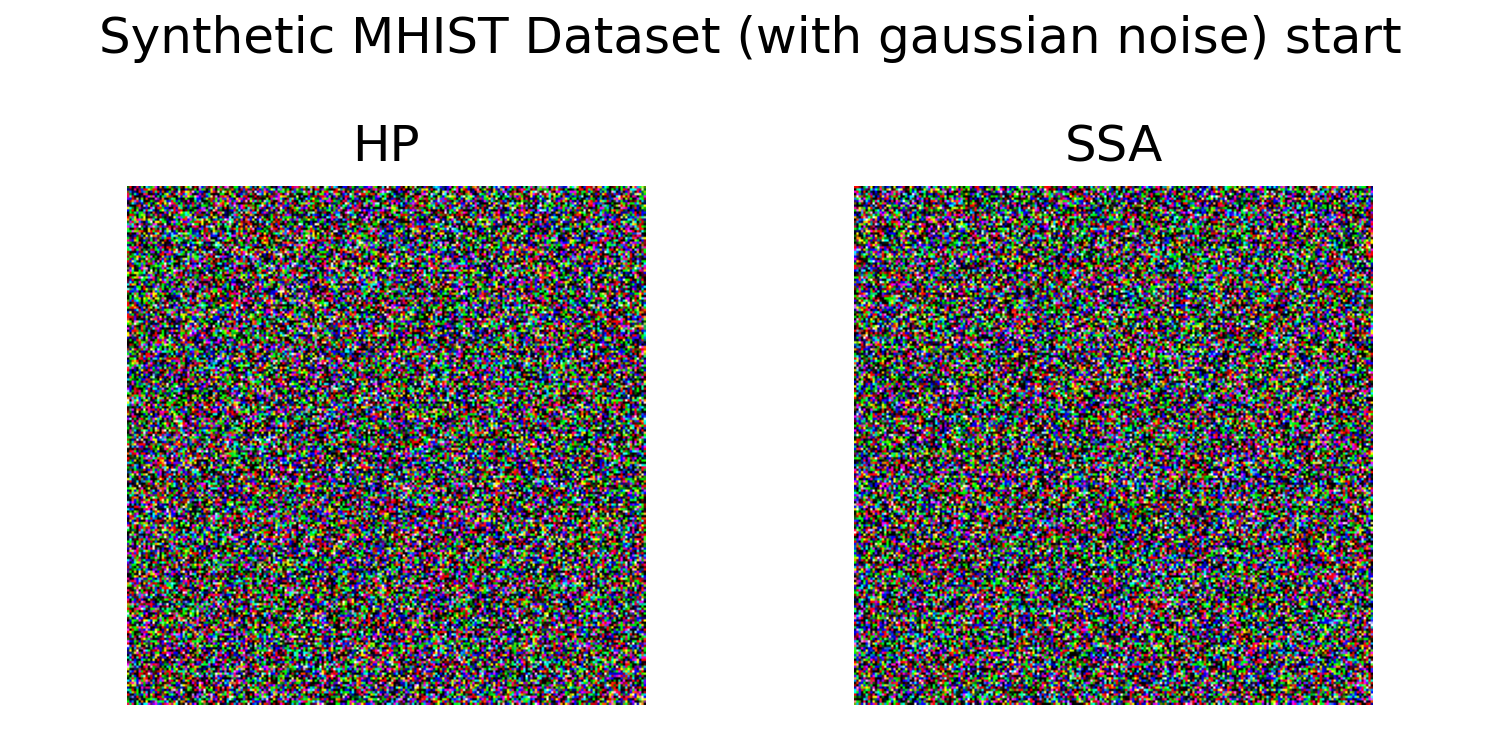
\includegraphics[width=0.48\textwidth]{mhist_noise_sample.png}
	\caption{Sample of Synthetic MHIST Dataset created from Gaussian noise (starting image)}
	\label{fig:mhist_noise_sample}
\end{figure}
\begin{figure}[H]
	\centering
	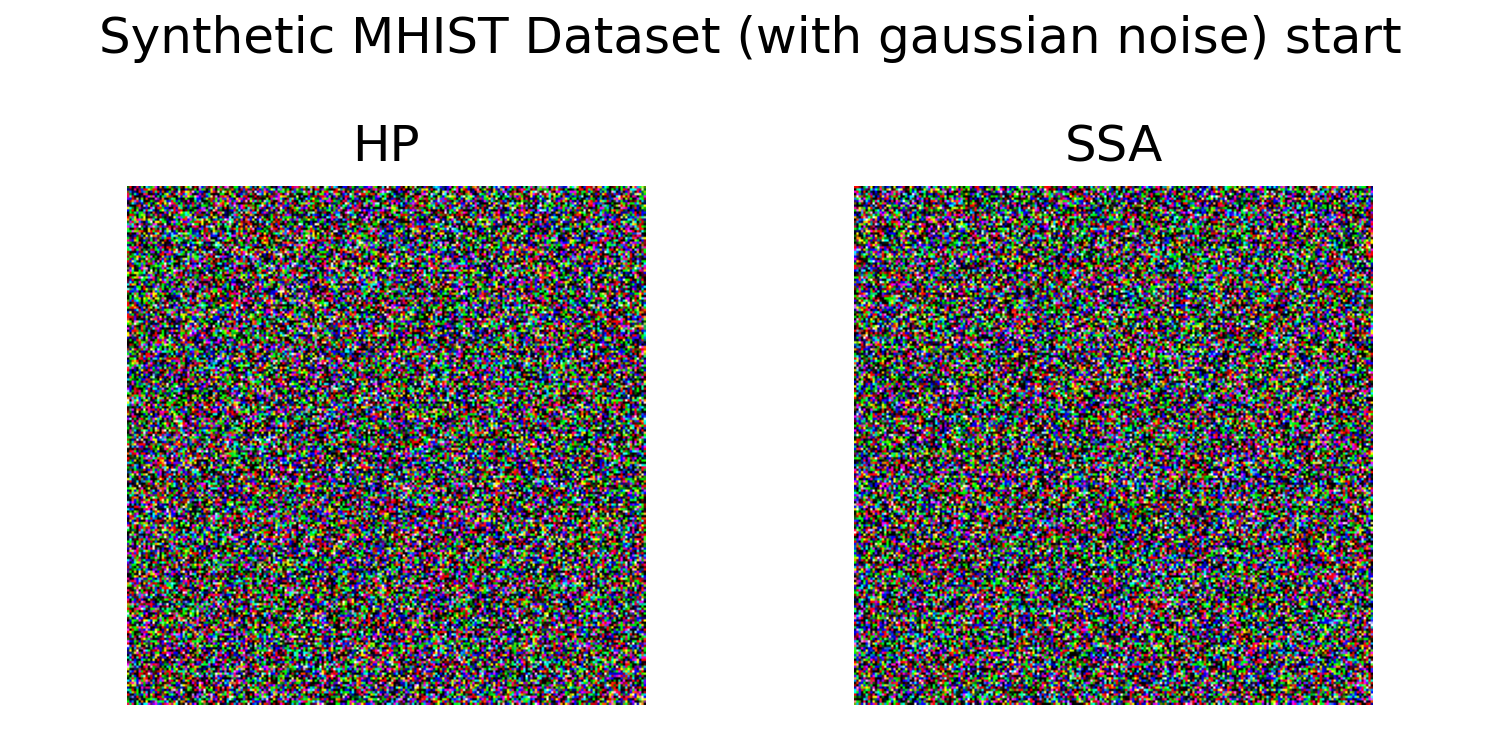
\includegraphics[width=0.48\textwidth]{mhist_noise_sample.png}
	\caption{Sample of Synthetic MHIST Dataset created from Gaussian noise(final image)}
	\label{fig:mhist_noise_final}
\end{figure}


\begin{figure}[H]
	\centering
	\includegraphics[width=0.48\textwidth]{mhist_noise_syn_all.png}
	\caption{Synthetic MHIST Dataset created from Gaussian noise}
	\label{fig:mhist_noise_syn_all}
\end{figure}

\subsubsection{ConvNet-7 using Synthetic Dataset}
\begin{figure}[H]
	\centering
	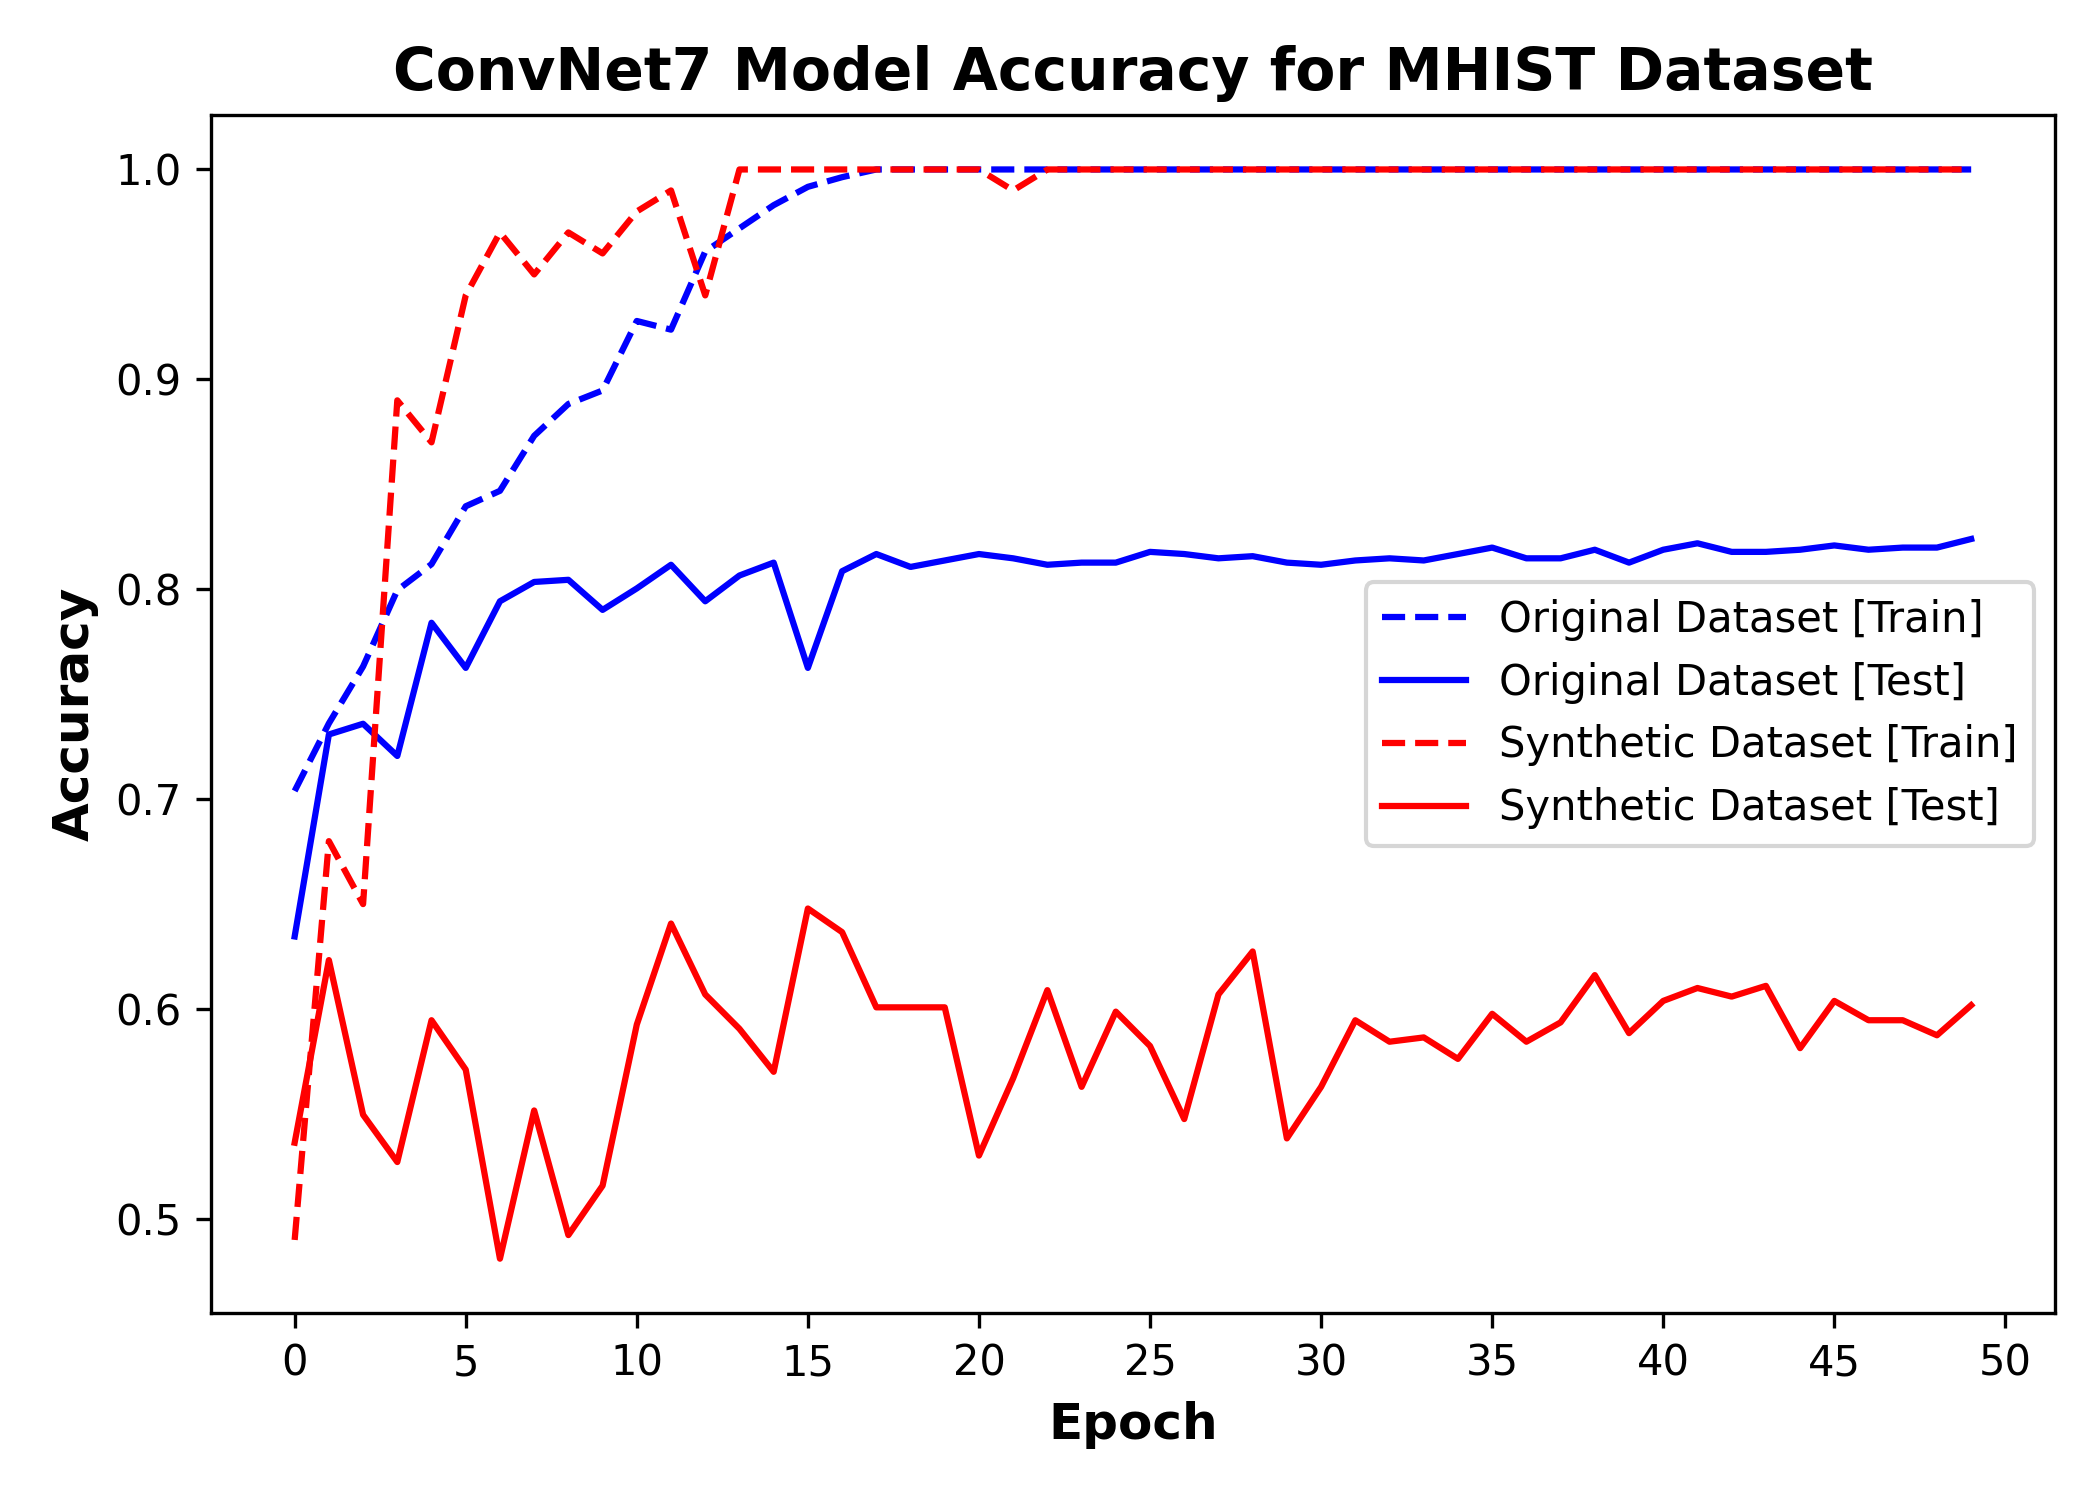
\includegraphics[width=0.48\textwidth]{mhist_syn_acc.png}
	\caption{ConvNet-7 Model Trained using Original and Synthetic dataset}
	\label{fig:mhist_syn_acc}
\end{figure}
\subsubsection{Cross-architecture Generalization - AlexNet}
\begin{figure}[H]
	\centering
	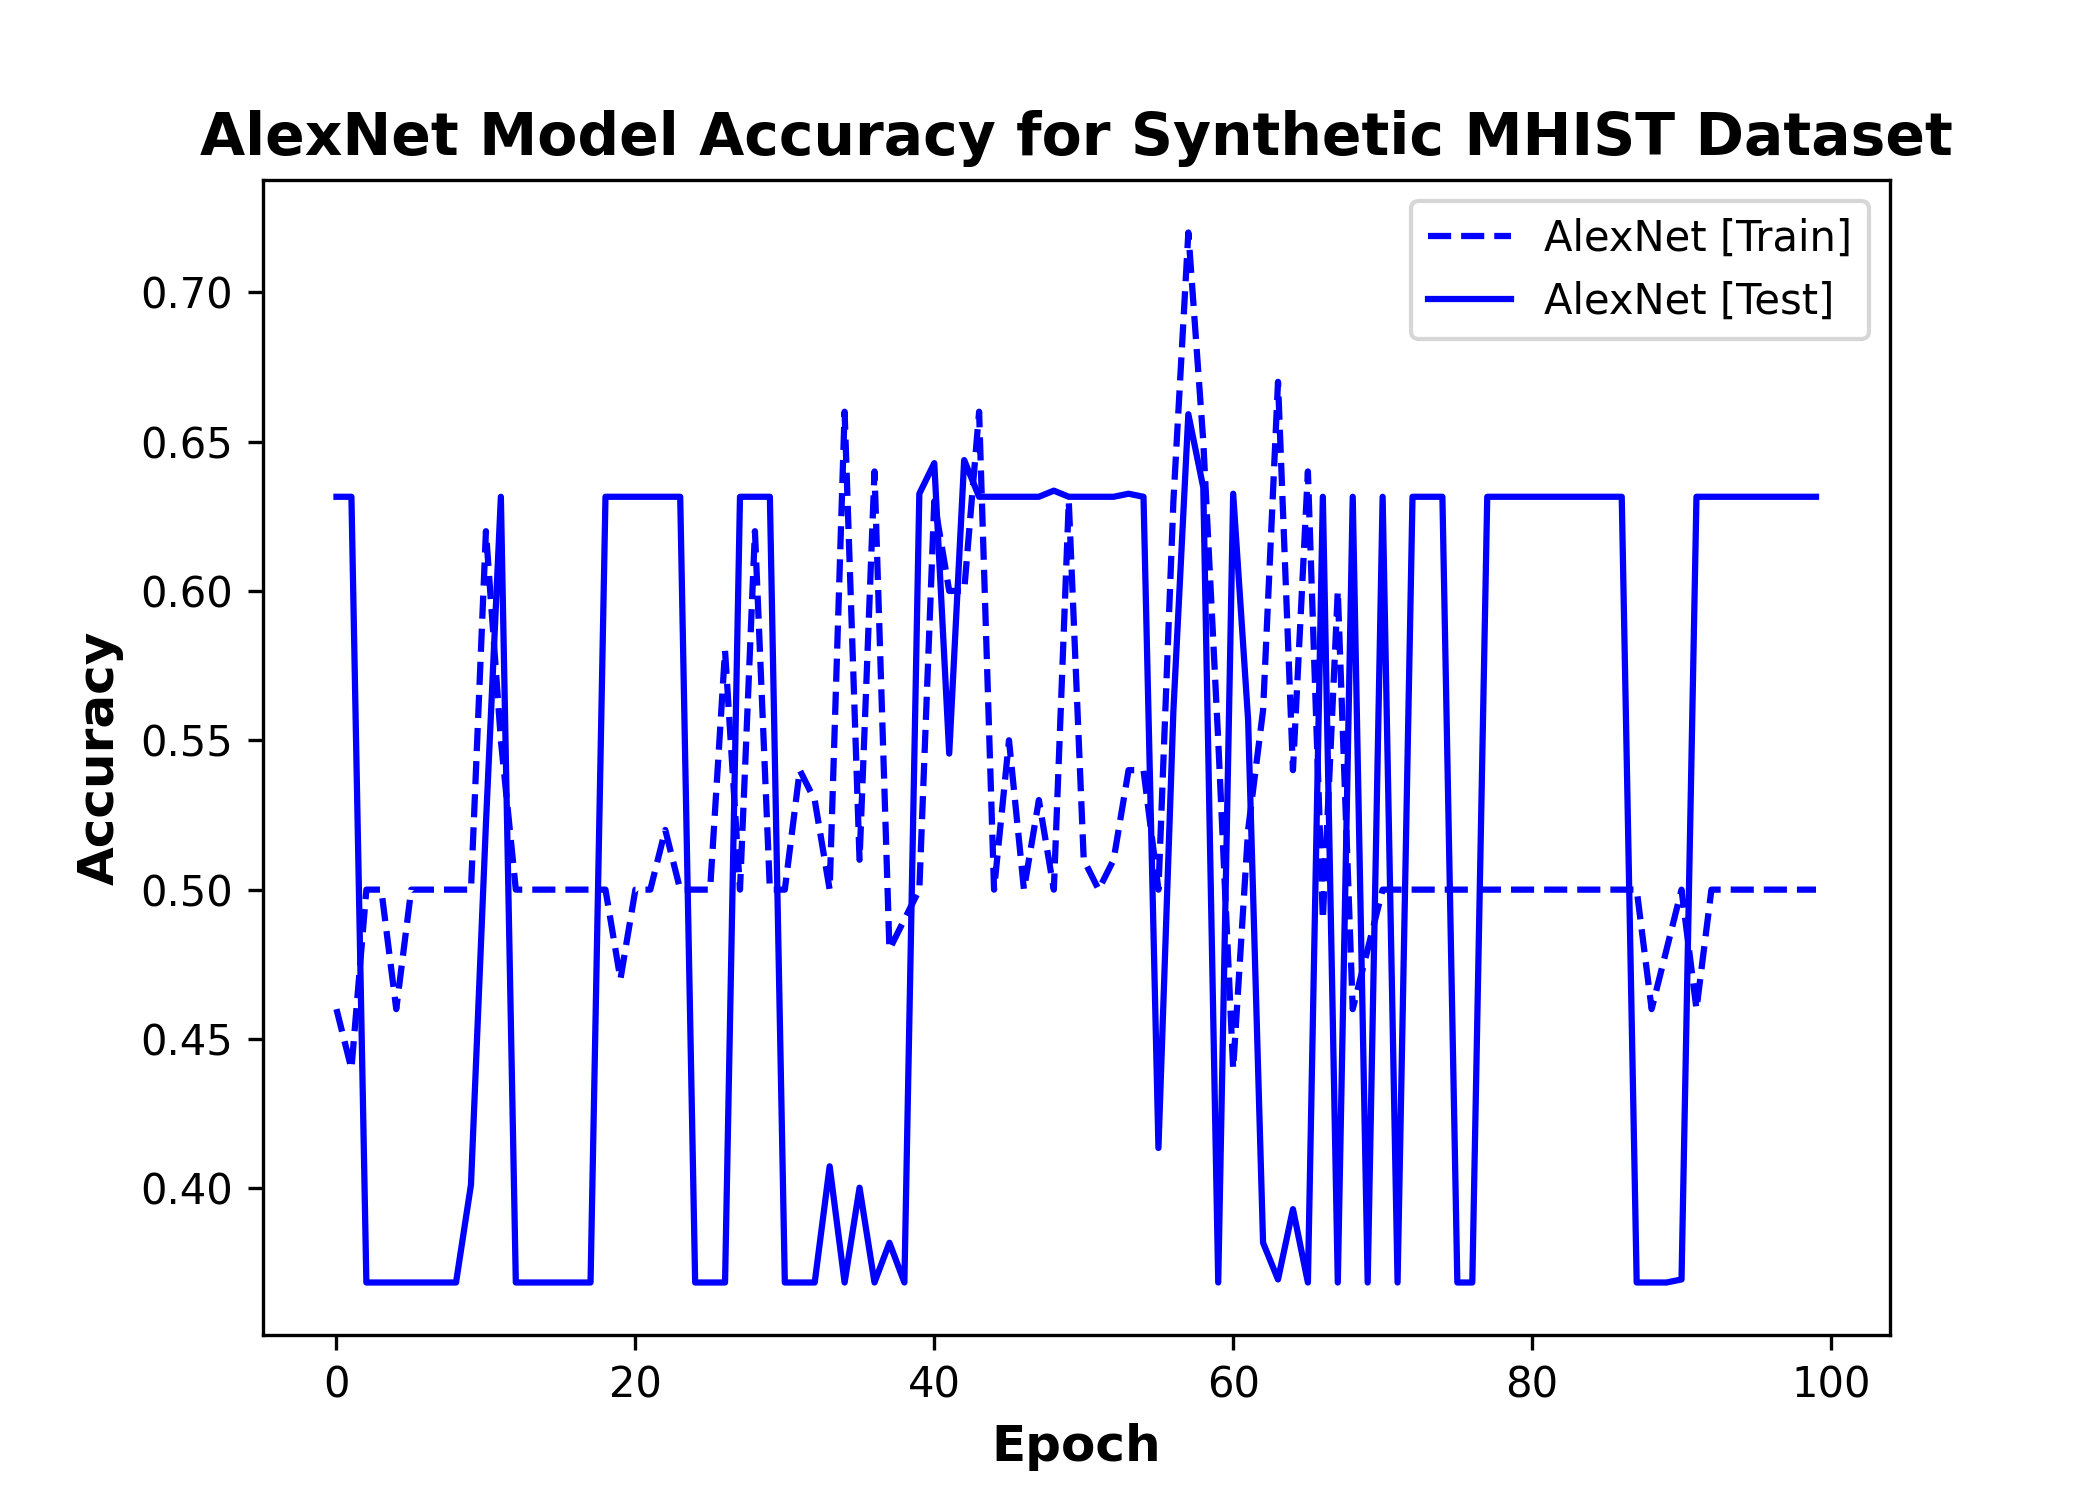
\includegraphics[width=0.48\textwidth]{mhist_alex_acc.png}
	\caption{AlexNet Model Trained using Synthetic dataset}
	\label{fig:mhist_alex_acc}
\end{figure}

\subsection{Data Distillation Application}
NAS with original dataset took 1607.3 seconds.
with synthetic dataset took 2.8 seconds.

\begin{figure}[H]
	\centering
	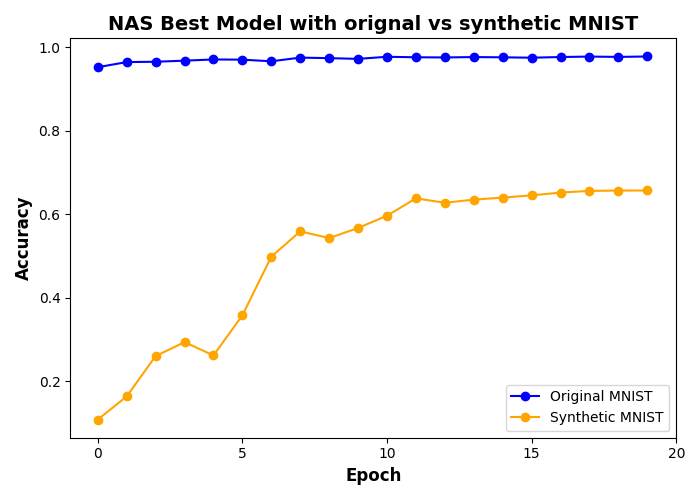
\includegraphics[width=0.48\textwidth]{nas_comparision.png}
	\caption{NAS best model with original vs synthetic MNIST dataset}
	\label{fig:nas_comparision}
\end{figure}
\section{Conclusion}

\section{References}
\nocite{*}
\printbibliography

\end{document}